\documentclass[a4paper]{book}
\usepackage{a4wide}
\usepackage{makeidx}
\usepackage{graphicx}
\usepackage{multicol}
\usepackage{float}
\usepackage{listings}
\usepackage{color}
\usepackage{textcomp}
\usepackage{alltt}
\usepackage{times}
\usepackage{ifpdf}
\ifpdf
\usepackage[pdftex,
            pagebackref=true,
            colorlinks=true,
            linkcolor=blue,
            unicode
           ]{hyperref}
\else
\usepackage[ps2pdf,
            pagebackref=true,
            colorlinks=true,
            linkcolor=blue,
            unicode
           ]{hyperref}
\usepackage{pspicture}
\fi
\usepackage[utf8]{inputenc}
\usepackage{doxygen}
\lstset{language=C++,inputencoding=utf8,basicstyle=\footnotesize,breaklines=true,breakatwhitespace=true,tabsize=8,numbers=left }
\makeindex
\setcounter{tocdepth}{3}
\renewcommand{\footrulewidth}{0.4pt}
\begin{document}
\hypersetup{pageanchor=false}
\begin{titlepage}
\vspace*{7cm}
\begin{center}
{\Large ModFossaCpp \\[1ex]\large 0.1 }\\
\vspace*{1cm}
{\large Generated by Doxygen 1.7.1}\\
\vspace*{0.5cm}
{\small Mon Feb 4 2013 19:17:13}\\
\end{center}
\end{titlepage}
\clearemptydoublepage
\pagenumbering{roman}
\tableofcontents
\clearemptydoublepage
\pagenumbering{arabic}
\hypersetup{pageanchor=true}
\chapter{Directory Hierarchy}
\section{Directories}
This directory hierarchy is sorted roughly, but not completely, alphabetically:\begin{DoxyCompactList}
\item \contentsline{section}{src}{\pageref{dir_98b68debbc6508d45834b3bb27214053}}{}
\item \contentsline{section}{test}{\pageref{dir_f47ba75ba3d9edb7c81ce81b4ffc651f}}{}
\end{DoxyCompactList}

\chapter{Class Index}
\section{Class List}
Here are the classes, structs, unions and interfaces with brief descriptions:\begin{DoxyCompactList}
\item\contentsline{section}{\hyperlink{classConnection}{Connection} }{\pageref{classConnection}}{}
\item\contentsline{section}{\hyperlink{classConstantRateConstant}{ConstantRateConstant} }{\pageref{classConstantRateConstant}}{}
\item\contentsline{section}{\hyperlink{classConstantRateConstantTest}{ConstantRateConstantTest} (TestCase for ConstantRateContant )}{\pageref{classConstantRateConstantTest}}{}
\item\contentsline{section}{\hyperlink{classMarkovModel}{MarkovModel} (Class responsible for creating and storing information required to describe a markov model for an ion channel )}{\pageref{classMarkovModel}}{}
\item\contentsline{section}{\hyperlink{classModelDescription}{ModelDescription} }{\pageref{classModelDescription}}{}
\item\contentsline{section}{\hyperlink{classRateConstantBase}{RateConstantBase} (Abstract base class for RateConstants )}{\pageref{classRateConstantBase}}{}
\item\contentsline{section}{\hyperlink{classState}{State} }{\pageref{classState}}{}
\item\contentsline{section}{\hyperlink{classStateOfTheWorld}{StateOfTheWorld} }{\pageref{classStateOfTheWorld}}{}
\end{DoxyCompactList}

\chapter{File Index}
\section{File List}
Here is a list of all files with brief descriptions:\begin{DoxyCompactList}
\item\contentsline{section}{/home/gareth/git/modfossa/ModFossaCpp/src/\hyperlink{Connection_8h}{Connection.h} }{\pageref{Connection_8h}}{}
\item\contentsline{section}{/home/gareth/git/modfossa/ModFossaCpp/src/\hyperlink{ConstantRateConstant_8h}{ConstantRateConstant.h} }{\pageref{ConstantRateConstant_8h}}{}
\item\contentsline{section}{/home/gareth/git/modfossa/ModFossaCpp/src/\hyperlink{MarkovModel_8cpp}{MarkovModel.cpp} }{\pageref{MarkovModel_8cpp}}{}
\item\contentsline{section}{/home/gareth/git/modfossa/ModFossaCpp/src/\hyperlink{MarkovModel_8h}{MarkovModel.h} }{\pageref{MarkovModel_8h}}{}
\item\contentsline{section}{/home/gareth/git/modfossa/ModFossaCpp/src/\hyperlink{ModelDescription_8h}{ModelDescription.h} }{\pageref{ModelDescription_8h}}{}
\item\contentsline{section}{/home/gareth/git/modfossa/ModFossaCpp/src/\hyperlink{RateConstantBase_8cpp}{RateConstantBase.cpp} }{\pageref{RateConstantBase_8cpp}}{}
\item\contentsline{section}{/home/gareth/git/modfossa/ModFossaCpp/src/\hyperlink{RateConstantBase_8h}{RateConstantBase.h} }{\pageref{RateConstantBase_8h}}{}
\item\contentsline{section}{/home/gareth/git/modfossa/ModFossaCpp/src/\hyperlink{RateConstantType_8h}{RateConstantType.h} }{\pageref{RateConstantType_8h}}{}
\item\contentsline{section}{/home/gareth/git/modfossa/ModFossaCpp/src/\hyperlink{State_8cpp}{State.cpp} }{\pageref{State_8cpp}}{}
\item\contentsline{section}{/home/gareth/git/modfossa/ModFossaCpp/src/\hyperlink{State_8h}{State.h} }{\pageref{State_8h}}{}
\item\contentsline{section}{/home/gareth/git/modfossa/ModFossaCpp/src/\hyperlink{StateOfTheWorld_8cpp}{StateOfTheWorld.cpp} }{\pageref{StateOfTheWorld_8cpp}}{}
\item\contentsline{section}{/home/gareth/git/modfossa/ModFossaCpp/src/\hyperlink{StateOfTheWorld_8h}{StateOfTheWorld.h} }{\pageref{StateOfTheWorld_8h}}{}
\item\contentsline{section}{/home/gareth/git/modfossa/ModFossaCpp/test/\hyperlink{ConstantRateConstantTest_8cpp}{ConstantRateConstantTest.cpp} }{\pageref{ConstantRateConstantTest_8cpp}}{}
\end{DoxyCompactList}

\chapter{Directory Documentation}
\hypertarget{dir_98b68debbc6508d45834b3bb27214053}{
\section{/home/gareth/git/modfossa/ModFossaCpp/src/ Directory Reference}
\label{dir_98b68debbc6508d45834b3bb27214053}\index{/home/gareth/git/modfossa/ModFossaCpp/src/ Directory Reference@{/home/gareth/git/modfossa/ModFossaCpp/src/ Directory Reference}}
}


Directory dependency graph for /home/gareth/git/modfossa/ModFossaCpp/src/:\nopagebreak
\begin{figure}[H]
\begin{center}
\leavevmode
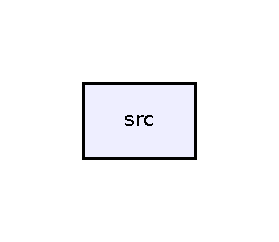
\includegraphics[width=134pt]{dir_98b68debbc6508d45834b3bb27214053_dep}
\end{center}
\end{figure}


\subsection*{Files}
\begin{DoxyCompactItemize}
\item 
file \hyperlink{Connection_8h}{Connection.h}
\item 
file \hyperlink{ConstantRateConstant_8h}{ConstantRateConstant.h}
\item 
file \hyperlink{MarkovModel_8cpp}{MarkovModel.cpp}
\item 
file \hyperlink{MarkovModel_8h}{MarkovModel.h}
\item 
file \hyperlink{ModelDescription_8h}{ModelDescription.h}
\item 
file \hyperlink{RateConstantBase_8cpp}{RateConstantBase.cpp}
\item 
file \hyperlink{RateConstantBase_8h}{RateConstantBase.h}
\item 
file \hyperlink{RateConstantType_8h}{RateConstantType.h}
\item 
file \hyperlink{State_8cpp}{State.cpp}
\item 
file \hyperlink{State_8h}{State.h}
\item 
file \hyperlink{StateOfTheWorld_8cpp}{StateOfTheWorld.cpp}
\item 
file \hyperlink{StateOfTheWorld_8h}{StateOfTheWorld.h}
\end{DoxyCompactItemize}

\hypertarget{dir_f47ba75ba3d9edb7c81ce81b4ffc651f}{
\section{/home/gareth/git/modfossa/ModFossaCpp/test/ Directory Reference}
\label{dir_f47ba75ba3d9edb7c81ce81b4ffc651f}\index{/home/gareth/git/modfossa/ModFossaCpp/test/ Directory Reference@{/home/gareth/git/modfossa/ModFossaCpp/test/ Directory Reference}}
}


Directory dependency graph for /home/gareth/git/modfossa/ModFossaCpp/test/:
\nopagebreak
\begin{figure}[H]
\begin{center}
\leavevmode
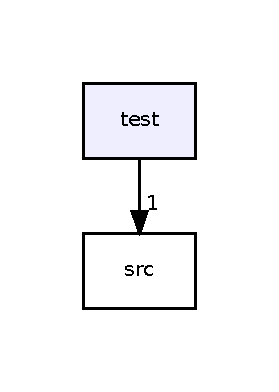
\includegraphics[width=134pt]{dir_f47ba75ba3d9edb7c81ce81b4ffc651f_dep}
\end{center}
\end{figure}


\subsection*{Files}
\begin{DoxyCompactItemize}
\item 
file \hyperlink{ConstantRateConstantTest_8cpp}{ConstantRateConstantTest.cpp}
\end{DoxyCompactItemize}

\chapter{Class Documentation}
\hypertarget{classConnection}{
\section{Connection Class Reference}
\label{classConnection}\index{Connection@{Connection}}
}


{\ttfamily \#include $<$Connection.h$>$}



Collaboration diagram for Connection:\nopagebreak
\begin{figure}[H]
\begin{center}
\leavevmode
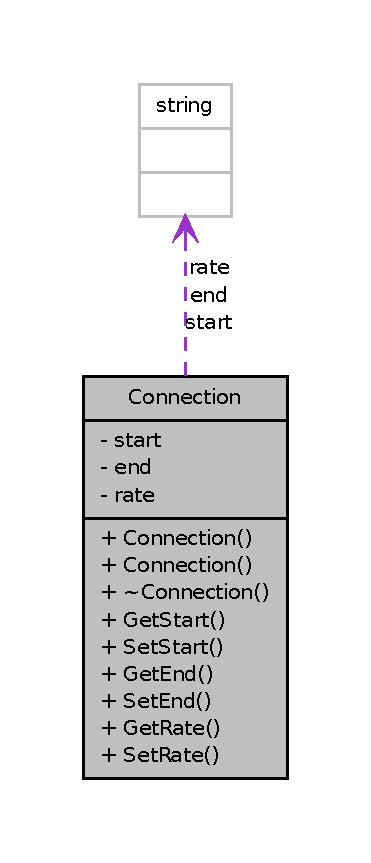
\includegraphics[width=178pt]{classConnection__coll__graph}
\end{center}
\end{figure}
\subsection*{Public Member Functions}
\begin{DoxyCompactItemize}
\item 
\hyperlink{classConnection_a9de94289ca6259f94ef6aeba3b134a77}{Connection} ()
\item 
\hyperlink{classConnection_ac63ae68b23cc60e56a5372f5d476d6b8}{Connection} (string \hyperlink{classConnection_a761d4f36c835443547758ee987454b4b}{start}, string \hyperlink{classConnection_aab791cc1d72139f7fce17ded6541037b}{end}, string \hyperlink{classConnection_a4169fd6525a547fa2fa238c58cf77dfe}{rate})
\item 
\hyperlink{classConnection_a2e4352edf667bea83001569e9da8a24d}{$\sim$Connection} ()
\item 
string \hyperlink{classConnection_adf469bc4ab33d4f426b39d2cf7d26b88}{GetStart} () const 
\item 
void \hyperlink{classConnection_acf6889ab6dc527abdc23a5d1aec8da49}{SetStart} (string)
\item 
string \hyperlink{classConnection_aab13bbdd6b7ada1d813d9ce7b3853a0b}{GetEnd} () const 
\item 
void \hyperlink{classConnection_a212339fd2842ca43b1bb4e53c0b5424e}{SetEnd} (string)
\item 
string \hyperlink{classConnection_a7551f3e3962a38598385e3ba57b5043f}{GetRate} () const 
\item 
void \hyperlink{classConnection_a402c8a961f2165fbcadc16ee9356d705}{SetRate} ()
\end{DoxyCompactItemize}
\subsection*{Private Attributes}
\begin{DoxyCompactItemize}
\item 
string \hyperlink{classConnection_a761d4f36c835443547758ee987454b4b}{start}
\item 
string \hyperlink{classConnection_aab791cc1d72139f7fce17ded6541037b}{end}
\item 
string \hyperlink{classConnection_a4169fd6525a547fa2fa238c58cf77dfe}{rate}
\end{DoxyCompactItemize}


\subsection{Detailed Description}


Definition at line 7 of file Connection.h.



\subsection{Constructor \& Destructor Documentation}
\hypertarget{classConnection_a9de94289ca6259f94ef6aeba3b134a77}{
\index{Connection@{Connection}!Connection@{Connection}}
\index{Connection@{Connection}!Connection@{Connection}}
\subsubsection[{Connection}]{\setlength{\rightskip}{0pt plus 5cm}Connection::Connection (
\begin{DoxyParamCaption}
{}
\end{DoxyParamCaption}
)}}
\label{classConnection_a9de94289ca6259f94ef6aeba3b134a77}
\hypertarget{classConnection_ac63ae68b23cc60e56a5372f5d476d6b8}{
\index{Connection@{Connection}!Connection@{Connection}}
\index{Connection@{Connection}!Connection@{Connection}}
\subsubsection[{Connection}]{\setlength{\rightskip}{0pt plus 5cm}Connection::Connection (
\begin{DoxyParamCaption}
\item[{string}]{ start, }
\item[{string}]{ end, }
\item[{string}]{ rate}
\end{DoxyParamCaption}
)}}
\label{classConnection_ac63ae68b23cc60e56a5372f5d476d6b8}
\hypertarget{classConnection_a2e4352edf667bea83001569e9da8a24d}{
\index{Connection@{Connection}!$\sim$Connection@{$\sim$Connection}}
\index{$\sim$Connection@{$\sim$Connection}!Connection@{Connection}}
\subsubsection[{$\sim$Connection}]{\setlength{\rightskip}{0pt plus 5cm}Connection::$\sim$Connection (
\begin{DoxyParamCaption}
{}
\end{DoxyParamCaption}
)}}
\label{classConnection_a2e4352edf667bea83001569e9da8a24d}


\subsection{Member Function Documentation}
\hypertarget{classConnection_aab13bbdd6b7ada1d813d9ce7b3853a0b}{
\index{Connection@{Connection}!GetEnd@{GetEnd}}
\index{GetEnd@{GetEnd}!Connection@{Connection}}
\subsubsection[{GetEnd}]{\setlength{\rightskip}{0pt plus 5cm}string Connection::GetEnd (
\begin{DoxyParamCaption}
{}
\end{DoxyParamCaption}
) const}}
\label{classConnection_aab13bbdd6b7ada1d813d9ce7b3853a0b}
\hypertarget{classConnection_a7551f3e3962a38598385e3ba57b5043f}{
\index{Connection@{Connection}!GetRate@{GetRate}}
\index{GetRate@{GetRate}!Connection@{Connection}}
\subsubsection[{GetRate}]{\setlength{\rightskip}{0pt plus 5cm}string Connection::GetRate (
\begin{DoxyParamCaption}
{}
\end{DoxyParamCaption}
) const}}
\label{classConnection_a7551f3e3962a38598385e3ba57b5043f}
\hypertarget{classConnection_adf469bc4ab33d4f426b39d2cf7d26b88}{
\index{Connection@{Connection}!GetStart@{GetStart}}
\index{GetStart@{GetStart}!Connection@{Connection}}
\subsubsection[{GetStart}]{\setlength{\rightskip}{0pt plus 5cm}string Connection::GetStart (
\begin{DoxyParamCaption}
{}
\end{DoxyParamCaption}
) const}}
\label{classConnection_adf469bc4ab33d4f426b39d2cf7d26b88}
\hypertarget{classConnection_a212339fd2842ca43b1bb4e53c0b5424e}{
\index{Connection@{Connection}!SetEnd@{SetEnd}}
\index{SetEnd@{SetEnd}!Connection@{Connection}}
\subsubsection[{SetEnd}]{\setlength{\rightskip}{0pt plus 5cm}void Connection::SetEnd (
\begin{DoxyParamCaption}
\item[{string}]{}
\end{DoxyParamCaption}
)}}
\label{classConnection_a212339fd2842ca43b1bb4e53c0b5424e}
\hypertarget{classConnection_a402c8a961f2165fbcadc16ee9356d705}{
\index{Connection@{Connection}!SetRate@{SetRate}}
\index{SetRate@{SetRate}!Connection@{Connection}}
\subsubsection[{SetRate}]{\setlength{\rightskip}{0pt plus 5cm}void Connection::SetRate (
\begin{DoxyParamCaption}
{}
\end{DoxyParamCaption}
)}}
\label{classConnection_a402c8a961f2165fbcadc16ee9356d705}
\hypertarget{classConnection_acf6889ab6dc527abdc23a5d1aec8da49}{
\index{Connection@{Connection}!SetStart@{SetStart}}
\index{SetStart@{SetStart}!Connection@{Connection}}
\subsubsection[{SetStart}]{\setlength{\rightskip}{0pt plus 5cm}void Connection::SetStart (
\begin{DoxyParamCaption}
\item[{string}]{}
\end{DoxyParamCaption}
)}}
\label{classConnection_acf6889ab6dc527abdc23a5d1aec8da49}


\subsection{Member Data Documentation}
\hypertarget{classConnection_aab791cc1d72139f7fce17ded6541037b}{
\index{Connection@{Connection}!end@{end}}
\index{end@{end}!Connection@{Connection}}
\subsubsection[{end}]{\setlength{\rightskip}{0pt plus 5cm}string {\bf Connection::end}\hspace{0.3cm}{\ttfamily  \mbox{[}private\mbox{]}}}}
\label{classConnection_aab791cc1d72139f7fce17ded6541037b}


Definition at line 22 of file Connection.h.

\hypertarget{classConnection_a4169fd6525a547fa2fa238c58cf77dfe}{
\index{Connection@{Connection}!rate@{rate}}
\index{rate@{rate}!Connection@{Connection}}
\subsubsection[{rate}]{\setlength{\rightskip}{0pt plus 5cm}string {\bf Connection::rate}\hspace{0.3cm}{\ttfamily  \mbox{[}private\mbox{]}}}}
\label{classConnection_a4169fd6525a547fa2fa238c58cf77dfe}


Definition at line 23 of file Connection.h.

\hypertarget{classConnection_a761d4f36c835443547758ee987454b4b}{
\index{Connection@{Connection}!start@{start}}
\index{start@{start}!Connection@{Connection}}
\subsubsection[{start}]{\setlength{\rightskip}{0pt plus 5cm}string {\bf Connection::start}\hspace{0.3cm}{\ttfamily  \mbox{[}private\mbox{]}}}}
\label{classConnection_a761d4f36c835443547758ee987454b4b}


Definition at line 21 of file Connection.h.



The documentation for this class was generated from the following file:\begin{DoxyCompactItemize}
\item 
/home/gareth/git/modfossa/ModFossaCpp/src/\hyperlink{Connection_8h}{Connection.h}\end{DoxyCompactItemize}

\hypertarget{classConstantRateConstant}{
\section{ConstantRateConstant Class Reference}
\label{classConstantRateConstant}\index{ConstantRateConstant@{ConstantRateConstant}}
}


{\ttfamily \#include $<$ConstantRateConstant.h$>$}



Collaboration diagram for ConstantRateConstant:\nopagebreak
\begin{figure}[H]
\begin{center}
\leavevmode
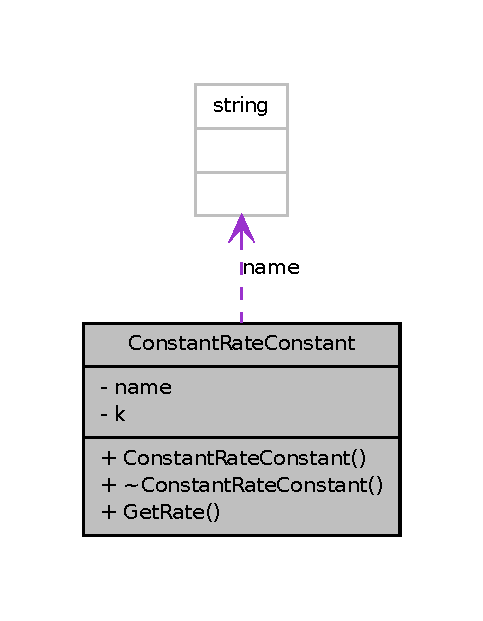
\includegraphics[width=232pt]{classConstantRateConstant__coll__graph}
\end{center}
\end{figure}
\subsection*{Public Member Functions}
\begin{DoxyCompactItemize}
\item 
\hyperlink{classConstantRateConstant_a733e712ecf33371ee2789b3f3f106d16}{ConstantRateConstant} (string \hyperlink{classConstantRateConstant_a303c84bba3e050f01322c05b55b34779}{name}, double \hyperlink{classConstantRateConstant_ac2963bcbd62887ad682c3f20464f5db1}{k})
\item 
virual \hyperlink{classConstantRateConstant_acf3c4ecdf09e328ea315eea945e1f2d4}{$\sim$ConstantRateConstant} ()
\item 
virtual double \hyperlink{classConstantRateConstant_ac74c67f5398dcaccda857b4417ea0ad3}{GetRate} (\hyperlink{classStateOfTheWorld}{StateOfTheWorld} $\ast$stateOfTheWorld)
\end{DoxyCompactItemize}
\subsection*{Private Attributes}
\begin{DoxyCompactItemize}
\item 
const string \hyperlink{classConstantRateConstant_a303c84bba3e050f01322c05b55b34779}{name}
\item 
const double \hyperlink{classConstantRateConstant_ac2963bcbd62887ad682c3f20464f5db1}{k}
\end{DoxyCompactItemize}


\subsection{Detailed Description}


Definition at line 9 of file ConstantRateConstant.h.



\subsection{Constructor \& Destructor Documentation}
\hypertarget{classConstantRateConstant_a733e712ecf33371ee2789b3f3f106d16}{
\index{ConstantRateConstant@{ConstantRateConstant}!ConstantRateConstant@{ConstantRateConstant}}
\index{ConstantRateConstant@{ConstantRateConstant}!ConstantRateConstant@{ConstantRateConstant}}
\subsubsection[{ConstantRateConstant}]{\setlength{\rightskip}{0pt plus 5cm}ConstantRateConstant::ConstantRateConstant (
\begin{DoxyParamCaption}
\item[{string}]{ name, }
\item[{double}]{ k}
\end{DoxyParamCaption}
)}}
\label{classConstantRateConstant_a733e712ecf33371ee2789b3f3f106d16}
\hypertarget{classConstantRateConstant_acf3c4ecdf09e328ea315eea945e1f2d4}{
\index{ConstantRateConstant@{ConstantRateConstant}!$\sim$ConstantRateConstant@{$\sim$ConstantRateConstant}}
\index{$\sim$ConstantRateConstant@{$\sim$ConstantRateConstant}!ConstantRateConstant@{ConstantRateConstant}}
\subsubsection[{$\sim$ConstantRateConstant}]{\setlength{\rightskip}{0pt plus 5cm}virual ConstantRateConstant::$\sim$ConstantRateConstant (
\begin{DoxyParamCaption}
{}
\end{DoxyParamCaption}
)}}
\label{classConstantRateConstant_acf3c4ecdf09e328ea315eea945e1f2d4}


\subsection{Member Function Documentation}
\hypertarget{classConstantRateConstant_ac74c67f5398dcaccda857b4417ea0ad3}{
\index{ConstantRateConstant@{ConstantRateConstant}!GetRate@{GetRate}}
\index{GetRate@{GetRate}!ConstantRateConstant@{ConstantRateConstant}}
\subsubsection[{GetRate}]{\setlength{\rightskip}{0pt plus 5cm}virtual double ConstantRateConstant::GetRate (
\begin{DoxyParamCaption}
\item[{{\bf StateOfTheWorld} $\ast$}]{ stateOfTheWorld}
\end{DoxyParamCaption}
)\hspace{0.3cm}{\ttfamily  \mbox{[}virtual\mbox{]}}}}
\label{classConstantRateConstant_ac74c67f5398dcaccda857b4417ea0ad3}


\subsection{Member Data Documentation}
\hypertarget{classConstantRateConstant_ac2963bcbd62887ad682c3f20464f5db1}{
\index{ConstantRateConstant@{ConstantRateConstant}!k@{k}}
\index{k@{k}!ConstantRateConstant@{ConstantRateConstant}}
\subsubsection[{k}]{\setlength{\rightskip}{0pt plus 5cm}const double {\bf ConstantRateConstant::k}\hspace{0.3cm}{\ttfamily  \mbox{[}private\mbox{]}}}}
\label{classConstantRateConstant_ac2963bcbd62887ad682c3f20464f5db1}


Definition at line 18 of file ConstantRateConstant.h.

\hypertarget{classConstantRateConstant_a303c84bba3e050f01322c05b55b34779}{
\index{ConstantRateConstant@{ConstantRateConstant}!name@{name}}
\index{name@{name}!ConstantRateConstant@{ConstantRateConstant}}
\subsubsection[{name}]{\setlength{\rightskip}{0pt plus 5cm}const string {\bf ConstantRateConstant::name}\hspace{0.3cm}{\ttfamily  \mbox{[}private\mbox{]}}}}
\label{classConstantRateConstant_a303c84bba3e050f01322c05b55b34779}


Definition at line 17 of file ConstantRateConstant.h.



The documentation for this class was generated from the following file:\begin{DoxyCompactItemize}
\item 
/home/gareth/git/modfossa/ModFossaCpp/src/\hyperlink{ConstantRateConstant_8h}{ConstantRateConstant.h}\end{DoxyCompactItemize}

\hypertarget{classConstantRateConstantTest}{
\section{ConstantRateConstantTest Class Reference}
\label{classConstantRateConstantTest}\index{ConstantRateConstantTest@{ConstantRateConstantTest}}
}


TestCase for ConstantRateContant.  




Collaboration diagram for ConstantRateConstantTest:
\nopagebreak
\begin{figure}[H]
\begin{center}
\leavevmode
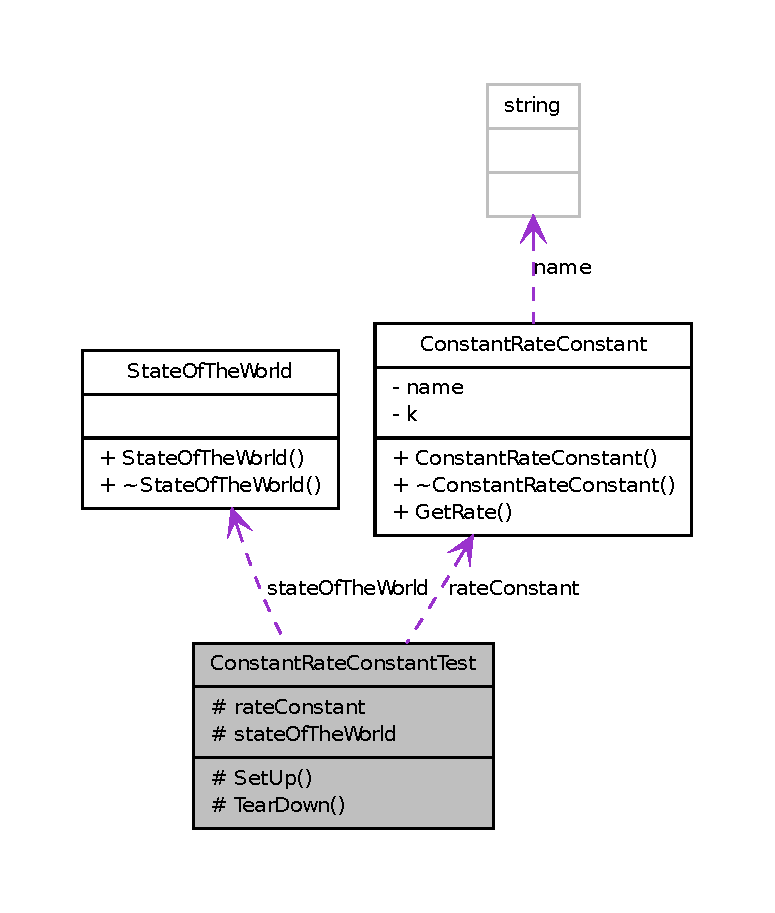
\includegraphics[width=372pt]{classConstantRateConstantTest__coll__graph}
\end{center}
\end{figure}
\subsection*{Protected Member Functions}
\begin{DoxyCompactItemize}
\item 
virtual void \hyperlink{classConstantRateConstantTest_afafa5788d27fda84c1a11c283e44407e}{SetUp} ()
\item 
virtual void \hyperlink{classConstantRateConstantTest_a7a77df51f310b128a6a9540a380be390}{TearDown} ()
\end{DoxyCompactItemize}
\subsection*{Protected Attributes}
\begin{DoxyCompactItemize}
\item 
\hyperlink{classConstantRateConstant}{ConstantRateConstant} $\ast$ \hyperlink{classConstantRateConstantTest_a3c05de2c151ba6f66f7bb4263a737b0e}{rateConstant}
\item 
\hyperlink{classStateOfTheWorld}{StateOfTheWorld} $\ast$ \hyperlink{classConstantRateConstantTest_a33885d8292d148c391de69acf60a882d}{stateOfTheWorld}
\end{DoxyCompactItemize}


\subsection{Detailed Description}
TestCase for ConstantRateContant. We test the constructor, and the GetRate() method under both normal and unnormal parameters. 

Definition at line 10 of file ConstantRateConstantTest.cpp.



\subsection{Member Function Documentation}
\hypertarget{classConstantRateConstantTest_afafa5788d27fda84c1a11c283e44407e}{
\index{ConstantRateConstantTest@{ConstantRateConstantTest}!SetUp@{SetUp}}
\index{SetUp@{SetUp}!ConstantRateConstantTest@{ConstantRateConstantTest}}
\subsubsection[{SetUp}]{\setlength{\rightskip}{0pt plus 5cm}virtual void ConstantRateConstantTest::SetUp (
\begin{DoxyParamCaption}
{}
\end{DoxyParamCaption}
)\hspace{0.3cm}{\ttfamily  \mbox{[}inline, protected, virtual\mbox{]}}}}
\label{classConstantRateConstantTest_afafa5788d27fda84c1a11c283e44407e}


Definition at line 5 of file ConstantRateConstantTest.cpp.

\hypertarget{classConstantRateConstantTest_a7a77df51f310b128a6a9540a380be390}{
\index{ConstantRateConstantTest@{ConstantRateConstantTest}!TearDown@{TearDown}}
\index{TearDown@{TearDown}!ConstantRateConstantTest@{ConstantRateConstantTest}}
\subsubsection[{TearDown}]{\setlength{\rightskip}{0pt plus 5cm}virtual void ConstantRateConstantTest::TearDown (
\begin{DoxyParamCaption}
{}
\end{DoxyParamCaption}
)\hspace{0.3cm}{\ttfamily  \mbox{[}inline, protected, virtual\mbox{]}}}}
\label{classConstantRateConstantTest_a7a77df51f310b128a6a9540a380be390}


Definition at line 9 of file ConstantRateConstantTest.cpp.



\subsection{Member Data Documentation}
\hypertarget{classConstantRateConstantTest_a3c05de2c151ba6f66f7bb4263a737b0e}{
\index{ConstantRateConstantTest@{ConstantRateConstantTest}!rateConstant@{rateConstant}}
\index{rateConstant@{rateConstant}!ConstantRateConstantTest@{ConstantRateConstantTest}}
\subsubsection[{rateConstant}]{\setlength{\rightskip}{0pt plus 5cm}{\bf ConstantRateConstant}$\ast$ {\bf ConstantRateConstantTest::rateConstant}\hspace{0.3cm}{\ttfamily  \mbox{[}protected\mbox{]}}}}
\label{classConstantRateConstantTest_a3c05de2c151ba6f66f7bb4263a737b0e}


Definition at line 13 of file ConstantRateConstantTest.cpp.

\hypertarget{classConstantRateConstantTest_a33885d8292d148c391de69acf60a882d}{
\index{ConstantRateConstantTest@{ConstantRateConstantTest}!stateOfTheWorld@{stateOfTheWorld}}
\index{stateOfTheWorld@{stateOfTheWorld}!ConstantRateConstantTest@{ConstantRateConstantTest}}
\subsubsection[{stateOfTheWorld}]{\setlength{\rightskip}{0pt plus 5cm}{\bf StateOfTheWorld}$\ast$ {\bf ConstantRateConstantTest::stateOfTheWorld}\hspace{0.3cm}{\ttfamily  \mbox{[}protected\mbox{]}}}}
\label{classConstantRateConstantTest_a33885d8292d148c391de69acf60a882d}


Definition at line 14 of file ConstantRateConstantTest.cpp.



The documentation for this class was generated from the following file:\begin{DoxyCompactItemize}
\item 
/home/gareth/git/modfossa/ModFossaCpp/test/\hyperlink{ConstantRateConstantTest_8cpp}{ConstantRateConstantTest.cpp}\end{DoxyCompactItemize}

\hypertarget{classMarkovModel}{
\section{MarkovModel Class Reference}
\label{classMarkovModel}\index{MarkovModel@{MarkovModel}}
}


Class responsible for creating and storing information required to describe a markov model for an ion channel.  




{\ttfamily \#include $<$MarkovModel.h$>$}



Collaboration diagram for MarkovModel:\nopagebreak
\begin{figure}[H]
\begin{center}
\leavevmode
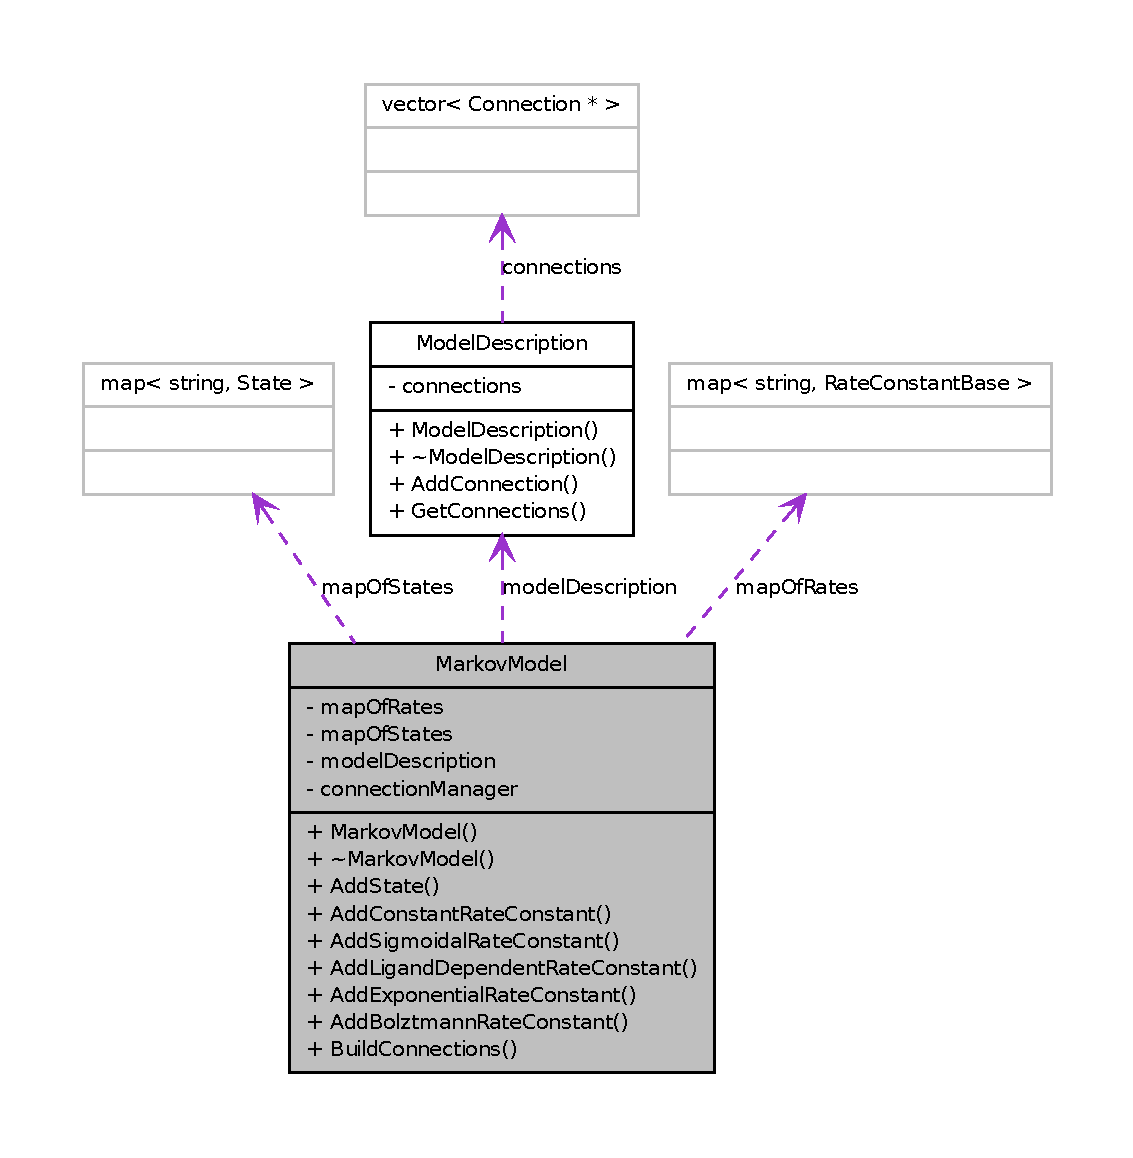
\includegraphics[width=400pt]{classMarkovModel__coll__graph}
\end{center}
\end{figure}
\subsection*{Public Member Functions}
\begin{DoxyCompactItemize}
\item 
\hyperlink{classMarkovModel_a78d9bb5082c4ca6d073d3f85b5724ec6}{MarkovModel} ()
\item 
\hyperlink{classMarkovModel_a793d422bad65797be59bc498b5244ccd}{$\sim$MarkovModel} ()
\item 
void \hyperlink{classMarkovModel_a05ee51096db3a9e5f99023a95f3a94c2}{AddState} (string name, bool conducting, bool initial=false)
\item 
void \hyperlink{classMarkovModel_a3a745b51845e7f2e143865a0e9b9b5c9}{AddConstantRateConstant} (string name, double k)
\item 
void \hyperlink{classMarkovModel_a6fd9d54968966763f121864765e1520a}{AddSigmoidalRateConstant} (string name, double a, double vHalf, double k)
\item 
void \hyperlink{classMarkovModel_a11a2021632cec3e65dd42fde69624b0c}{AddLigandDependentRateConstant} (string name, double k, double ligandPower, string ligandAbbreviation)
\item 
void \hyperlink{classMarkovModel_afb18b6980e5240e59d1f9fb334c95256}{AddExponentialRateConstant} (string name, double a, double k)
\item 
void \hyperlink{classMarkovModel_a387e958195aa614d0c8210f1e12abb31}{AddBolztmannRateConstant} (string name, double a, double a2, double vHalf, double k)
\item 
void \hyperlink{classMarkovModel_a059fde492604827abdf90fcd32889f5c}{BuildConnections} ()
\end{DoxyCompactItemize}
\subsection*{Private Attributes}
\begin{DoxyCompactItemize}
\item 
map$<$ string, \hyperlink{classRateConstantBase}{RateConstantBase} $>$ \hyperlink{classMarkovModel_aacb8c8d6db1b31efeb05947a1421426e}{mapOfRates}
\item 
map$<$ string, \hyperlink{classState}{State} $>$ \hyperlink{classMarkovModel_a291cff9e856b3b348fbee694c344c219}{mapOfStates}
\item 
\hyperlink{classModelDescription}{ModelDescription} $\ast$ \hyperlink{classMarkovModel_acb12261525cf0a48bb92d10078a94fbc}{modelDescription}
\item 
ConnectionManager $\ast$ \hyperlink{classMarkovModel_a1cb9169b2ffa849a71aeb4c65411505b}{connectionManager}
\end{DoxyCompactItemize}


\subsection{Detailed Description}
Class responsible for creating and storing information required to describe a markov model for an ion channel. The user adds RateConstants and States using the methods provided. After the model is described, the user calls \hyperlink{classMarkovModel_a059fde492604827abdf90fcd32889f5c}{BuildConnections()}. At this point the ConnectionManager and \hyperlink{classModelDescription}{ModelDescription} are used to create the transitionMatrix, which is used to run the simulation. 

Definition at line 23 of file MarkovModel.h.



\subsection{Constructor \& Destructor Documentation}
\hypertarget{classMarkovModel_a78d9bb5082c4ca6d073d3f85b5724ec6}{
\index{MarkovModel@{MarkovModel}!MarkovModel@{MarkovModel}}
\index{MarkovModel@{MarkovModel}!MarkovModel@{MarkovModel}}
\subsubsection[{MarkovModel}]{\setlength{\rightskip}{0pt plus 5cm}MarkovModel::MarkovModel (
\begin{DoxyParamCaption}
\item[{void}]{}
\end{DoxyParamCaption}
)}}
\label{classMarkovModel_a78d9bb5082c4ca6d073d3f85b5724ec6}


Definition at line 4 of file MarkovModel.cpp.

\hypertarget{classMarkovModel_a793d422bad65797be59bc498b5244ccd}{
\index{MarkovModel@{MarkovModel}!$\sim$MarkovModel@{$\sim$MarkovModel}}
\index{$\sim$MarkovModel@{$\sim$MarkovModel}!MarkovModel@{MarkovModel}}
\subsubsection[{$\sim$MarkovModel}]{\setlength{\rightskip}{0pt plus 5cm}MarkovModel::$\sim$MarkovModel (
\begin{DoxyParamCaption}
\item[{void}]{}
\end{DoxyParamCaption}
)}}
\label{classMarkovModel_a793d422bad65797be59bc498b5244ccd}


Definition at line 9 of file MarkovModel.cpp.



\subsection{Member Function Documentation}
\hypertarget{classMarkovModel_a387e958195aa614d0c8210f1e12abb31}{
\index{MarkovModel@{MarkovModel}!AddBolztmannRateConstant@{AddBolztmannRateConstant}}
\index{AddBolztmannRateConstant@{AddBolztmannRateConstant}!MarkovModel@{MarkovModel}}
\subsubsection[{AddBolztmannRateConstant}]{\setlength{\rightskip}{0pt plus 5cm}void MarkovModel::AddBolztmannRateConstant (
\begin{DoxyParamCaption}
\item[{string}]{ name, }
\item[{double}]{ a, }
\item[{double}]{ a2, }
\item[{double}]{ vHalf, }
\item[{double}]{ k}
\end{DoxyParamCaption}
)}}
\label{classMarkovModel_a387e958195aa614d0c8210f1e12abb31}
\hypertarget{classMarkovModel_a3a745b51845e7f2e143865a0e9b9b5c9}{
\index{MarkovModel@{MarkovModel}!AddConstantRateConstant@{AddConstantRateConstant}}
\index{AddConstantRateConstant@{AddConstantRateConstant}!MarkovModel@{MarkovModel}}
\subsubsection[{AddConstantRateConstant}]{\setlength{\rightskip}{0pt plus 5cm}void MarkovModel::AddConstantRateConstant (
\begin{DoxyParamCaption}
\item[{string}]{ name, }
\item[{double}]{ k}
\end{DoxyParamCaption}
)}}
\label{classMarkovModel_a3a745b51845e7f2e143865a0e9b9b5c9}
\hypertarget{classMarkovModel_afb18b6980e5240e59d1f9fb334c95256}{
\index{MarkovModel@{MarkovModel}!AddExponentialRateConstant@{AddExponentialRateConstant}}
\index{AddExponentialRateConstant@{AddExponentialRateConstant}!MarkovModel@{MarkovModel}}
\subsubsection[{AddExponentialRateConstant}]{\setlength{\rightskip}{0pt plus 5cm}void MarkovModel::AddExponentialRateConstant (
\begin{DoxyParamCaption}
\item[{string}]{ name, }
\item[{double}]{ a, }
\item[{double}]{ k}
\end{DoxyParamCaption}
)}}
\label{classMarkovModel_afb18b6980e5240e59d1f9fb334c95256}
\hypertarget{classMarkovModel_a11a2021632cec3e65dd42fde69624b0c}{
\index{MarkovModel@{MarkovModel}!AddLigandDependentRateConstant@{AddLigandDependentRateConstant}}
\index{AddLigandDependentRateConstant@{AddLigandDependentRateConstant}!MarkovModel@{MarkovModel}}
\subsubsection[{AddLigandDependentRateConstant}]{\setlength{\rightskip}{0pt plus 5cm}void MarkovModel::AddLigandDependentRateConstant (
\begin{DoxyParamCaption}
\item[{string}]{ name, }
\item[{double}]{ k, }
\item[{double}]{ ligandPower, }
\item[{string}]{ ligandAbbreviation}
\end{DoxyParamCaption}
)}}
\label{classMarkovModel_a11a2021632cec3e65dd42fde69624b0c}
\hypertarget{classMarkovModel_a6fd9d54968966763f121864765e1520a}{
\index{MarkovModel@{MarkovModel}!AddSigmoidalRateConstant@{AddSigmoidalRateConstant}}
\index{AddSigmoidalRateConstant@{AddSigmoidalRateConstant}!MarkovModel@{MarkovModel}}
\subsubsection[{AddSigmoidalRateConstant}]{\setlength{\rightskip}{0pt plus 5cm}void MarkovModel::AddSigmoidalRateConstant (
\begin{DoxyParamCaption}
\item[{string}]{ name, }
\item[{double}]{ a, }
\item[{double}]{ vHalf, }
\item[{double}]{ k}
\end{DoxyParamCaption}
)}}
\label{classMarkovModel_a6fd9d54968966763f121864765e1520a}
\hypertarget{classMarkovModel_a05ee51096db3a9e5f99023a95f3a94c2}{
\index{MarkovModel@{MarkovModel}!AddState@{AddState}}
\index{AddState@{AddState}!MarkovModel@{MarkovModel}}
\subsubsection[{AddState}]{\setlength{\rightskip}{0pt plus 5cm}void MarkovModel::AddState (
\begin{DoxyParamCaption}
\item[{string}]{ name, }
\item[{bool}]{ conducting, }
\item[{bool}]{ initial = {\ttfamily false}}
\end{DoxyParamCaption}
)}}
\label{classMarkovModel_a05ee51096db3a9e5f99023a95f3a94c2}
\hypertarget{classMarkovModel_a059fde492604827abdf90fcd32889f5c}{
\index{MarkovModel@{MarkovModel}!BuildConnections@{BuildConnections}}
\index{BuildConnections@{BuildConnections}!MarkovModel@{MarkovModel}}
\subsubsection[{BuildConnections}]{\setlength{\rightskip}{0pt plus 5cm}void MarkovModel::BuildConnections (
\begin{DoxyParamCaption}
{}
\end{DoxyParamCaption}
)}}
\label{classMarkovModel_a059fde492604827abdf90fcd32889f5c}


\subsection{Member Data Documentation}
\hypertarget{classMarkovModel_a1cb9169b2ffa849a71aeb4c65411505b}{
\index{MarkovModel@{MarkovModel}!connectionManager@{connectionManager}}
\index{connectionManager@{connectionManager}!MarkovModel@{MarkovModel}}
\subsubsection[{connectionManager}]{\setlength{\rightskip}{0pt plus 5cm}ConnectionManager$\ast$ {\bf MarkovModel::connectionManager}\hspace{0.3cm}{\ttfamily  \mbox{[}private\mbox{]}}}}
\label{classMarkovModel_a1cb9169b2ffa849a71aeb4c65411505b}


Definition at line 50 of file MarkovModel.h.

\hypertarget{classMarkovModel_aacb8c8d6db1b31efeb05947a1421426e}{
\index{MarkovModel@{MarkovModel}!mapOfRates@{mapOfRates}}
\index{mapOfRates@{mapOfRates}!MarkovModel@{MarkovModel}}
\subsubsection[{mapOfRates}]{\setlength{\rightskip}{0pt plus 5cm}map$<$string, {\bf RateConstantBase}$>$ {\bf MarkovModel::mapOfRates}\hspace{0.3cm}{\ttfamily  \mbox{[}private\mbox{]}}}}
\label{classMarkovModel_aacb8c8d6db1b31efeb05947a1421426e}


Definition at line 46 of file MarkovModel.h.

\hypertarget{classMarkovModel_a291cff9e856b3b348fbee694c344c219}{
\index{MarkovModel@{MarkovModel}!mapOfStates@{mapOfStates}}
\index{mapOfStates@{mapOfStates}!MarkovModel@{MarkovModel}}
\subsubsection[{mapOfStates}]{\setlength{\rightskip}{0pt plus 5cm}map$<$string, {\bf State}$>$ {\bf MarkovModel::mapOfStates}\hspace{0.3cm}{\ttfamily  \mbox{[}private\mbox{]}}}}
\label{classMarkovModel_a291cff9e856b3b348fbee694c344c219}


Definition at line 47 of file MarkovModel.h.

\hypertarget{classMarkovModel_acb12261525cf0a48bb92d10078a94fbc}{
\index{MarkovModel@{MarkovModel}!modelDescription@{modelDescription}}
\index{modelDescription@{modelDescription}!MarkovModel@{MarkovModel}}
\subsubsection[{modelDescription}]{\setlength{\rightskip}{0pt plus 5cm}{\bf ModelDescription}$\ast$ {\bf MarkovModel::modelDescription}\hspace{0.3cm}{\ttfamily  \mbox{[}private\mbox{]}}}}
\label{classMarkovModel_acb12261525cf0a48bb92d10078a94fbc}


Definition at line 49 of file MarkovModel.h.



The documentation for this class was generated from the following files:\begin{DoxyCompactItemize}
\item 
/home/gareth/git/modfossa/ModFossaCpp/src/\hyperlink{MarkovModel_8h}{MarkovModel.h}\item 
/home/gareth/git/modfossa/ModFossaCpp/src/\hyperlink{MarkovModel_8cpp}{MarkovModel.cpp}\end{DoxyCompactItemize}

\hypertarget{classModelDescription}{
\section{ModelDescription Class Reference}
\label{classModelDescription}\index{ModelDescription@{ModelDescription}}
}


{\ttfamily \#include $<$ModelDescription.h$>$}



Collaboration diagram for ModelDescription:\nopagebreak
\begin{figure}[H]
\begin{center}
\leavevmode
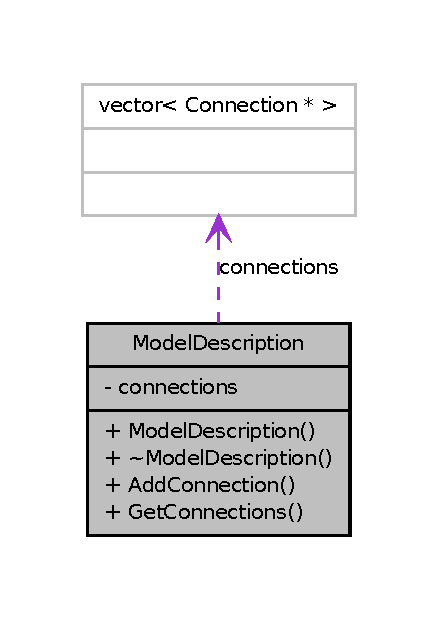
\includegraphics[width=210pt]{classModelDescription__coll__graph}
\end{center}
\end{figure}
\subsection*{Public Member Functions}
\begin{DoxyCompactItemize}
\item 
\hyperlink{classModelDescription_a7a1da1ba67e855968da674ec6a4e1d7a}{ModelDescription} ()
\item 
\hyperlink{classModelDescription_aae623832121ffc4ff0130012ca4b26a9}{$\sim$ModelDescription} ()
\item 
void \hyperlink{classModelDescription_a5eb05482f951226fe696d227cb5a60ff}{AddConnection} (string startState, string endState, string rateName)
\item 
const vector$<$ \hyperlink{classConnection}{Connection} $\ast$ $>$ \& \hyperlink{classModelDescription_a3849c1b405db870a7306aa00ceb625b4}{GetConnections} () const 
\end{DoxyCompactItemize}
\subsection*{Private Attributes}
\begin{DoxyCompactItemize}
\item 
vector$<$ \hyperlink{classConnection}{Connection} $\ast$ $>$ \hyperlink{classModelDescription_af6d01d5a79db737efefc24dabe6a76f8}{connections}
\end{DoxyCompactItemize}


\subsection{Detailed Description}


Definition at line 12 of file ModelDescription.h.



\subsection{Constructor \& Destructor Documentation}
\hypertarget{classModelDescription_a7a1da1ba67e855968da674ec6a4e1d7a}{
\index{ModelDescription@{ModelDescription}!ModelDescription@{ModelDescription}}
\index{ModelDescription@{ModelDescription}!ModelDescription@{ModelDescription}}
\subsubsection[{ModelDescription}]{\setlength{\rightskip}{0pt plus 5cm}ModelDescription::ModelDescription (
\begin{DoxyParamCaption}
{}
\end{DoxyParamCaption}
)}}
\label{classModelDescription_a7a1da1ba67e855968da674ec6a4e1d7a}
\hypertarget{classModelDescription_aae623832121ffc4ff0130012ca4b26a9}{
\index{ModelDescription@{ModelDescription}!$\sim$ModelDescription@{$\sim$ModelDescription}}
\index{$\sim$ModelDescription@{$\sim$ModelDescription}!ModelDescription@{ModelDescription}}
\subsubsection[{$\sim$ModelDescription}]{\setlength{\rightskip}{0pt plus 5cm}ModelDescription::$\sim$ModelDescription (
\begin{DoxyParamCaption}
{}
\end{DoxyParamCaption}
)}}
\label{classModelDescription_aae623832121ffc4ff0130012ca4b26a9}


\subsection{Member Function Documentation}
\hypertarget{classModelDescription_a5eb05482f951226fe696d227cb5a60ff}{
\index{ModelDescription@{ModelDescription}!AddConnection@{AddConnection}}
\index{AddConnection@{AddConnection}!ModelDescription@{ModelDescription}}
\subsubsection[{AddConnection}]{\setlength{\rightskip}{0pt plus 5cm}void ModelDescription::AddConnection (
\begin{DoxyParamCaption}
\item[{string}]{ startState, }
\item[{string}]{ endState, }
\item[{string}]{ rateName}
\end{DoxyParamCaption}
)}}
\label{classModelDescription_a5eb05482f951226fe696d227cb5a60ff}
\hypertarget{classModelDescription_a3849c1b405db870a7306aa00ceb625b4}{
\index{ModelDescription@{ModelDescription}!GetConnections@{GetConnections}}
\index{GetConnections@{GetConnections}!ModelDescription@{ModelDescription}}
\subsubsection[{GetConnections}]{\setlength{\rightskip}{0pt plus 5cm}const vector$<${\bf Connection}$\ast$$>$\& ModelDescription::GetConnections (
\begin{DoxyParamCaption}
{}
\end{DoxyParamCaption}
) const}}
\label{classModelDescription_a3849c1b405db870a7306aa00ceb625b4}


\subsection{Member Data Documentation}
\hypertarget{classModelDescription_af6d01d5a79db737efefc24dabe6a76f8}{
\index{ModelDescription@{ModelDescription}!connections@{connections}}
\index{connections@{connections}!ModelDescription@{ModelDescription}}
\subsubsection[{connections}]{\setlength{\rightskip}{0pt plus 5cm}vector$<${\bf Connection}$\ast$$>$ {\bf ModelDescription::connections}\hspace{0.3cm}{\ttfamily  \mbox{[}private\mbox{]}}}}
\label{classModelDescription_af6d01d5a79db737efefc24dabe6a76f8}


Definition at line 20 of file ModelDescription.h.



The documentation for this class was generated from the following file:\begin{DoxyCompactItemize}
\item 
/home/gareth/git/modfossa/ModFossaCpp/src/\hyperlink{ModelDescription_8h}{ModelDescription.h}\end{DoxyCompactItemize}

\hypertarget{classRateConstantBase}{
\section{RateConstantBase Class Reference}
\label{classRateConstantBase}\index{RateConstantBase@{RateConstantBase}}
}


Abstract base class for RateConstants.  




{\ttfamily \#include $<$RateConstantBase.h$>$}

\subsection*{Public Member Functions}
\begin{DoxyCompactItemize}
\item 
\hyperlink{classRateConstantBase_a56622d91aa9c54c4fd2202b5f09ac048}{RateConstantBase} ()
\item 
virtual \hyperlink{classRateConstantBase_a1d0bd28f65a52f8bf719b3282b6ca168}{$\sim$RateConstantBase} ()
\item 
virtual double \hyperlink{classRateConstantBase_ae71e41dedc24072fa19775ab065623f2}{GetRate} (\hyperlink{classStateOfTheWorld}{StateOfTheWorld} $\ast$stateOfTheWorld)=0
\end{DoxyCompactItemize}


\subsection{Detailed Description}
Abstract base class for RateConstants. 

Definition at line 12 of file RateConstantBase.h.



\subsection{Constructor \& Destructor Documentation}
\hypertarget{classRateConstantBase_a56622d91aa9c54c4fd2202b5f09ac048}{
\index{RateConstantBase@{RateConstantBase}!RateConstantBase@{RateConstantBase}}
\index{RateConstantBase@{RateConstantBase}!RateConstantBase@{RateConstantBase}}
\subsubsection[{RateConstantBase}]{\setlength{\rightskip}{0pt plus 5cm}RateConstantBase::RateConstantBase (
\begin{DoxyParamCaption}
\item[{void}]{}
\end{DoxyParamCaption}
)}}
\label{classRateConstantBase_a56622d91aa9c54c4fd2202b5f09ac048}


Definition at line 4 of file RateConstantBase.cpp.

\hypertarget{classRateConstantBase_a1d0bd28f65a52f8bf719b3282b6ca168}{
\index{RateConstantBase@{RateConstantBase}!$\sim$RateConstantBase@{$\sim$RateConstantBase}}
\index{$\sim$RateConstantBase@{$\sim$RateConstantBase}!RateConstantBase@{RateConstantBase}}
\subsubsection[{$\sim$RateConstantBase}]{\setlength{\rightskip}{0pt plus 5cm}RateConstantBase::$\sim$RateConstantBase (
\begin{DoxyParamCaption}
\item[{void}]{}
\end{DoxyParamCaption}
)\hspace{0.3cm}{\ttfamily  \mbox{[}virtual\mbox{]}}}}
\label{classRateConstantBase_a1d0bd28f65a52f8bf719b3282b6ca168}


Definition at line 9 of file RateConstantBase.cpp.



\subsection{Member Function Documentation}
\hypertarget{classRateConstantBase_ae71e41dedc24072fa19775ab065623f2}{
\index{RateConstantBase@{RateConstantBase}!GetRate@{GetRate}}
\index{GetRate@{GetRate}!RateConstantBase@{RateConstantBase}}
\subsubsection[{GetRate}]{\setlength{\rightskip}{0pt plus 5cm}virtual double RateConstantBase::GetRate (
\begin{DoxyParamCaption}
\item[{{\bf StateOfTheWorld} $\ast$}]{ stateOfTheWorld}
\end{DoxyParamCaption}
)\hspace{0.3cm}{\ttfamily  \mbox{[}pure virtual\mbox{]}}}}
\label{classRateConstantBase_ae71e41dedc24072fa19775ab065623f2}


The documentation for this class was generated from the following files:\begin{DoxyCompactItemize}
\item 
/home/gareth/git/modfossa/ModFossaCpp/src/\hyperlink{RateConstantBase_8h}{RateConstantBase.h}\item 
/home/gareth/git/modfossa/ModFossaCpp/src/\hyperlink{RateConstantBase_8cpp}{RateConstantBase.cpp}\end{DoxyCompactItemize}

\hypertarget{classState}{
\section{State Class Reference}
\label{classState}\index{State@{State}}
}


{\ttfamily \#include $<$State.h$>$}



Collaboration diagram for State:\nopagebreak
\begin{figure}[H]
\begin{center}
\leavevmode
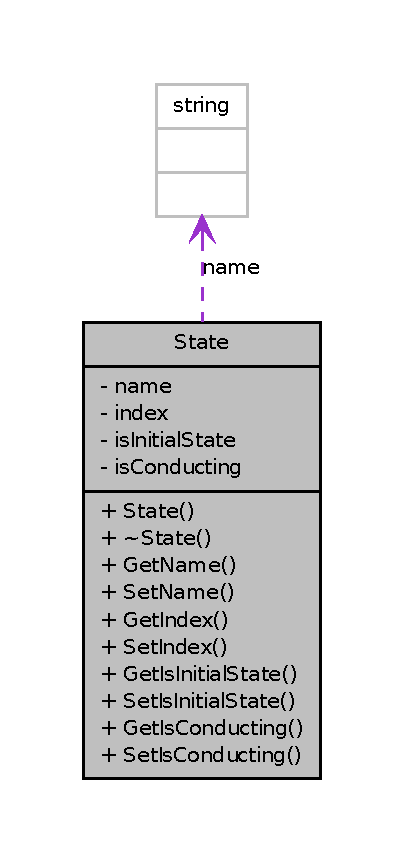
\includegraphics[width=194pt]{classState__coll__graph}
\end{center}
\end{figure}
\subsection*{Public Member Functions}
\begin{DoxyCompactItemize}
\item 
\hyperlink{classState_ab91bb1dd5aa6260ab2a456581daf9ec2}{State} ()
\item 
\hyperlink{classState_afab438d92b90dc18d194dbd9c9c8bab3}{$\sim$State} ()
\item 
std::string \hyperlink{classState_a53d7c7ca3f4bbd4ed057d34bfffbaab3}{GetName} () const 
\item 
void \hyperlink{classState_a0aa838bac877e885a40846b40f7fb3f7}{SetName} (std::string \hyperlink{classState_ad57f19fd0a86f129840d8739253d2c72}{name})
\item 
int \hyperlink{classState_a0df5da1bbb6f418694ce5f789ca7e6c5}{GetIndex} () const 
\item 
void \hyperlink{classState_a0a366542e4e8f21aed25152ee7cea6be}{SetIndex} (int \hyperlink{classState_a91451f2d71245fba7cfe1d2ff248c13c}{index})
\item 
bool \hyperlink{classState_ad70ea5b882eb85376b91acd0fd89ad0f}{GetIsInitialState} () const 
\item 
void \hyperlink{classState_a3d6b9ceac51f4c063628ba5708db926a}{SetIsInitialState} (bool \hyperlink{classState_a3f648ae24fee45cce26ce51bbe93deb4}{isInitialState})
\item 
bool \hyperlink{classState_a25100298e536317fd0f6d53220a017a7}{GetIsConducting} () const 
\item 
void \hyperlink{classState_aba42323ab4cf1fe314181fcdd3273acf}{SetIsConducting} (bool \hyperlink{classState_a5d20171d44b393ae9bad5cd61d1e8f45}{isConducting})
\end{DoxyCompactItemize}
\subsection*{Private Attributes}
\begin{DoxyCompactItemize}
\item 
std::string \hyperlink{classState_ad57f19fd0a86f129840d8739253d2c72}{name}
\item 
int \hyperlink{classState_a91451f2d71245fba7cfe1d2ff248c13c}{index}
\item 
bool \hyperlink{classState_a3f648ae24fee45cce26ce51bbe93deb4}{isInitialState}
\item 
bool \hyperlink{classState_a5d20171d44b393ae9bad5cd61d1e8f45}{isConducting}
\end{DoxyCompactItemize}


\subsection{Detailed Description}


Definition at line 6 of file State.h.



\subsection{Constructor \& Destructor Documentation}
\hypertarget{classState_ab91bb1dd5aa6260ab2a456581daf9ec2}{
\index{State@{State}!State@{State}}
\index{State@{State}!State@{State}}
\subsubsection[{State}]{\setlength{\rightskip}{0pt plus 5cm}State::State (
\begin{DoxyParamCaption}
\item[{void}]{}
\end{DoxyParamCaption}
)}}
\label{classState_ab91bb1dd5aa6260ab2a456581daf9ec2}


Definition at line 4 of file State.cpp.

\hypertarget{classState_afab438d92b90dc18d194dbd9c9c8bab3}{
\index{State@{State}!$\sim$State@{$\sim$State}}
\index{$\sim$State@{$\sim$State}!State@{State}}
\subsubsection[{$\sim$State}]{\setlength{\rightskip}{0pt plus 5cm}State::$\sim$State (
\begin{DoxyParamCaption}
\item[{void}]{}
\end{DoxyParamCaption}
)}}
\label{classState_afab438d92b90dc18d194dbd9c9c8bab3}


Definition at line 9 of file State.cpp.



\subsection{Member Function Documentation}
\hypertarget{classState_a0df5da1bbb6f418694ce5f789ca7e6c5}{
\index{State@{State}!GetIndex@{GetIndex}}
\index{GetIndex@{GetIndex}!State@{State}}
\subsubsection[{GetIndex}]{\setlength{\rightskip}{0pt plus 5cm}int State::GetIndex (
\begin{DoxyParamCaption}
{}
\end{DoxyParamCaption}
) const}}
\label{classState_a0df5da1bbb6f418694ce5f789ca7e6c5}
\hypertarget{classState_a25100298e536317fd0f6d53220a017a7}{
\index{State@{State}!GetIsConducting@{GetIsConducting}}
\index{GetIsConducting@{GetIsConducting}!State@{State}}
\subsubsection[{GetIsConducting}]{\setlength{\rightskip}{0pt plus 5cm}bool State::GetIsConducting (
\begin{DoxyParamCaption}
{}
\end{DoxyParamCaption}
) const}}
\label{classState_a25100298e536317fd0f6d53220a017a7}
\hypertarget{classState_ad70ea5b882eb85376b91acd0fd89ad0f}{
\index{State@{State}!GetIsInitialState@{GetIsInitialState}}
\index{GetIsInitialState@{GetIsInitialState}!State@{State}}
\subsubsection[{GetIsInitialState}]{\setlength{\rightskip}{0pt plus 5cm}bool State::GetIsInitialState (
\begin{DoxyParamCaption}
{}
\end{DoxyParamCaption}
) const}}
\label{classState_ad70ea5b882eb85376b91acd0fd89ad0f}
\hypertarget{classState_a53d7c7ca3f4bbd4ed057d34bfffbaab3}{
\index{State@{State}!GetName@{GetName}}
\index{GetName@{GetName}!State@{State}}
\subsubsection[{GetName}]{\setlength{\rightskip}{0pt plus 5cm}std::string State::GetName (
\begin{DoxyParamCaption}
{}
\end{DoxyParamCaption}
) const}}
\label{classState_a53d7c7ca3f4bbd4ed057d34bfffbaab3}
\hypertarget{classState_a0a366542e4e8f21aed25152ee7cea6be}{
\index{State@{State}!SetIndex@{SetIndex}}
\index{SetIndex@{SetIndex}!State@{State}}
\subsubsection[{SetIndex}]{\setlength{\rightskip}{0pt plus 5cm}void State::SetIndex (
\begin{DoxyParamCaption}
\item[{int}]{ index}
\end{DoxyParamCaption}
)}}
\label{classState_a0a366542e4e8f21aed25152ee7cea6be}
\hypertarget{classState_aba42323ab4cf1fe314181fcdd3273acf}{
\index{State@{State}!SetIsConducting@{SetIsConducting}}
\index{SetIsConducting@{SetIsConducting}!State@{State}}
\subsubsection[{SetIsConducting}]{\setlength{\rightskip}{0pt plus 5cm}void State::SetIsConducting (
\begin{DoxyParamCaption}
\item[{bool}]{ isConducting}
\end{DoxyParamCaption}
)}}
\label{classState_aba42323ab4cf1fe314181fcdd3273acf}
\hypertarget{classState_a3d6b9ceac51f4c063628ba5708db926a}{
\index{State@{State}!SetIsInitialState@{SetIsInitialState}}
\index{SetIsInitialState@{SetIsInitialState}!State@{State}}
\subsubsection[{SetIsInitialState}]{\setlength{\rightskip}{0pt plus 5cm}void State::SetIsInitialState (
\begin{DoxyParamCaption}
\item[{bool}]{ isInitialState}
\end{DoxyParamCaption}
)}}
\label{classState_a3d6b9ceac51f4c063628ba5708db926a}
\hypertarget{classState_a0aa838bac877e885a40846b40f7fb3f7}{
\index{State@{State}!SetName@{SetName}}
\index{SetName@{SetName}!State@{State}}
\subsubsection[{SetName}]{\setlength{\rightskip}{0pt plus 5cm}void State::SetName (
\begin{DoxyParamCaption}
\item[{std::string}]{ name}
\end{DoxyParamCaption}
)}}
\label{classState_a0aa838bac877e885a40846b40f7fb3f7}


\subsection{Member Data Documentation}
\hypertarget{classState_a91451f2d71245fba7cfe1d2ff248c13c}{
\index{State@{State}!index@{index}}
\index{index@{index}!State@{State}}
\subsubsection[{index}]{\setlength{\rightskip}{0pt plus 5cm}int {\bf State::index}\hspace{0.3cm}{\ttfamily  \mbox{[}private\mbox{]}}}}
\label{classState_a91451f2d71245fba7cfe1d2ff248c13c}


Definition at line 26 of file State.h.

\hypertarget{classState_a5d20171d44b393ae9bad5cd61d1e8f45}{
\index{State@{State}!isConducting@{isConducting}}
\index{isConducting@{isConducting}!State@{State}}
\subsubsection[{isConducting}]{\setlength{\rightskip}{0pt plus 5cm}bool {\bf State::isConducting}\hspace{0.3cm}{\ttfamily  \mbox{[}private\mbox{]}}}}
\label{classState_a5d20171d44b393ae9bad5cd61d1e8f45}


Definition at line 28 of file State.h.

\hypertarget{classState_a3f648ae24fee45cce26ce51bbe93deb4}{
\index{State@{State}!isInitialState@{isInitialState}}
\index{isInitialState@{isInitialState}!State@{State}}
\subsubsection[{isInitialState}]{\setlength{\rightskip}{0pt plus 5cm}bool {\bf State::isInitialState}\hspace{0.3cm}{\ttfamily  \mbox{[}private\mbox{]}}}}
\label{classState_a3f648ae24fee45cce26ce51bbe93deb4}


Definition at line 27 of file State.h.

\hypertarget{classState_ad57f19fd0a86f129840d8739253d2c72}{
\index{State@{State}!name@{name}}
\index{name@{name}!State@{State}}
\subsubsection[{name}]{\setlength{\rightskip}{0pt plus 5cm}std::string {\bf State::name}\hspace{0.3cm}{\ttfamily  \mbox{[}private\mbox{]}}}}
\label{classState_ad57f19fd0a86f129840d8739253d2c72}


Definition at line 25 of file State.h.



The documentation for this class was generated from the following files:\begin{DoxyCompactItemize}
\item 
/home/gareth/git/modfossa/ModFossaCpp/src/\hyperlink{State_8h}{State.h}\item 
/home/gareth/git/modfossa/ModFossaCpp/src/\hyperlink{State_8cpp}{State.cpp}\end{DoxyCompactItemize}

\hypertarget{classStateOfTheWorld}{
\section{StateOfTheWorld Class Reference}
\label{classStateOfTheWorld}\index{StateOfTheWorld@{StateOfTheWorld}}
}


{\ttfamily \#include $<$StateOfTheWorld.h$>$}

\subsection*{Public Member Functions}
\begin{DoxyCompactItemize}
\item 
\hyperlink{classStateOfTheWorld_ae10cd514a40d11acdfb34b414d37c8ac}{StateOfTheWorld} ()
\item 
\hyperlink{classStateOfTheWorld_a4dc3e3ab8f0ab40240145fafab13a4d2}{$\sim$StateOfTheWorld} ()
\end{DoxyCompactItemize}


\subsection{Detailed Description}


Definition at line 4 of file StateOfTheWorld.h.



\subsection{Constructor \& Destructor Documentation}
\hypertarget{classStateOfTheWorld_ae10cd514a40d11acdfb34b414d37c8ac}{
\index{StateOfTheWorld@{StateOfTheWorld}!StateOfTheWorld@{StateOfTheWorld}}
\index{StateOfTheWorld@{StateOfTheWorld}!StateOfTheWorld@{StateOfTheWorld}}
\subsubsection[{StateOfTheWorld}]{\setlength{\rightskip}{0pt plus 5cm}StateOfTheWorld::StateOfTheWorld (
\begin{DoxyParamCaption}
\item[{void}]{}
\end{DoxyParamCaption}
)}}
\label{classStateOfTheWorld_ae10cd514a40d11acdfb34b414d37c8ac}


Definition at line 4 of file StateOfTheWorld.cpp.

\hypertarget{classStateOfTheWorld_a4dc3e3ab8f0ab40240145fafab13a4d2}{
\index{StateOfTheWorld@{StateOfTheWorld}!$\sim$StateOfTheWorld@{$\sim$StateOfTheWorld}}
\index{$\sim$StateOfTheWorld@{$\sim$StateOfTheWorld}!StateOfTheWorld@{StateOfTheWorld}}
\subsubsection[{$\sim$StateOfTheWorld}]{\setlength{\rightskip}{0pt plus 5cm}StateOfTheWorld::$\sim$StateOfTheWorld (
\begin{DoxyParamCaption}
\item[{void}]{}
\end{DoxyParamCaption}
)}}
\label{classStateOfTheWorld_a4dc3e3ab8f0ab40240145fafab13a4d2}


Definition at line 9 of file StateOfTheWorld.cpp.



The documentation for this class was generated from the following files:\begin{DoxyCompactItemize}
\item 
/home/gareth/git/modfossa/ModFossaCpp/src/\hyperlink{StateOfTheWorld_8h}{StateOfTheWorld.h}\item 
/home/gareth/git/modfossa/ModFossaCpp/src/\hyperlink{StateOfTheWorld_8cpp}{StateOfTheWorld.cpp}\end{DoxyCompactItemize}

\chapter{File Documentation}
\hypertarget{Connection_8h}{
\section{/home/gareth/git/modfossa/ModFossaCpp/src/Connection.h File Reference}
\label{Connection_8h}\index{/home/gareth/git/modfossa/ModFossaCpp/src/Connection.h@{/home/gareth/git/modfossa/ModFossaCpp/src/Connection.h}}
}
{\ttfamily \#include $<$string$>$}\par
Include dependency graph for Connection.h:\nopagebreak
\begin{figure}[H]
\begin{center}
\leavevmode
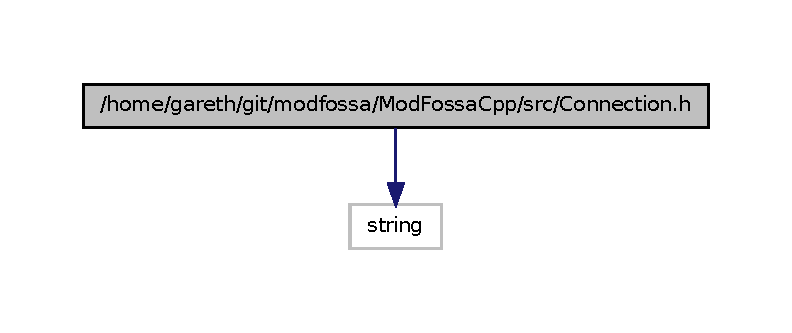
\includegraphics[width=380pt]{Connection_8h__incl}
\end{center}
\end{figure}
\subsection*{Classes}
\begin{DoxyCompactItemize}
\item 
class \hyperlink{classConnection}{Connection}
\end{DoxyCompactItemize}

\hypertarget{ConstantRateConstant_8h}{
\section{/home/gareth/git/modfossa/ModFossaCpp/src/ConstantRateConstant.h File Reference}
\label{ConstantRateConstant_8h}\index{/home/gareth/git/modfossa/ModFossaCpp/src/ConstantRateConstant.h@{/home/gareth/git/modfossa/ModFossaCpp/src/ConstantRateConstant.h}}
}
{\ttfamily \#include \char`\"{}RateConstantBase.h\char`\"{}}\par
{\ttfamily \#include $<$string$>$}\par
Include dependency graph for ConstantRateConstant.h:\nopagebreak
\begin{figure}[H]
\begin{center}
\leavevmode
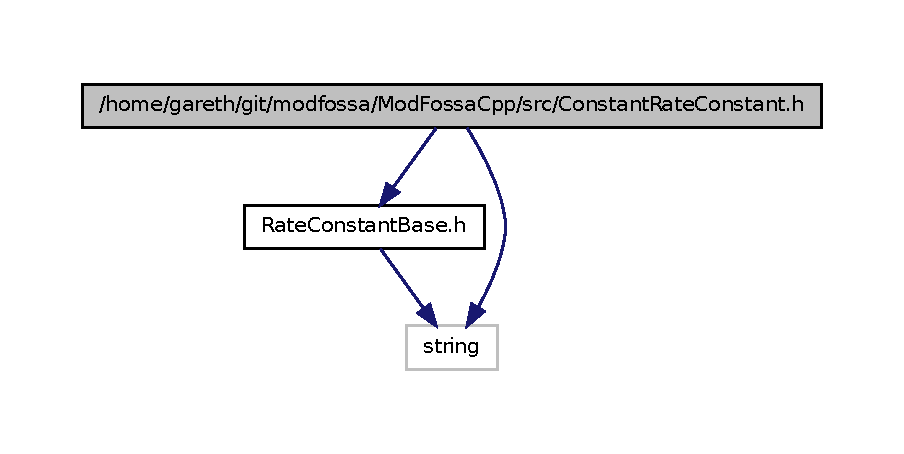
\includegraphics[width=400pt]{ConstantRateConstant_8h__incl}
\end{center}
\end{figure}
This graph shows which files directly or indirectly include this file:
\nopagebreak
\begin{figure}[H]
\begin{center}
\leavevmode
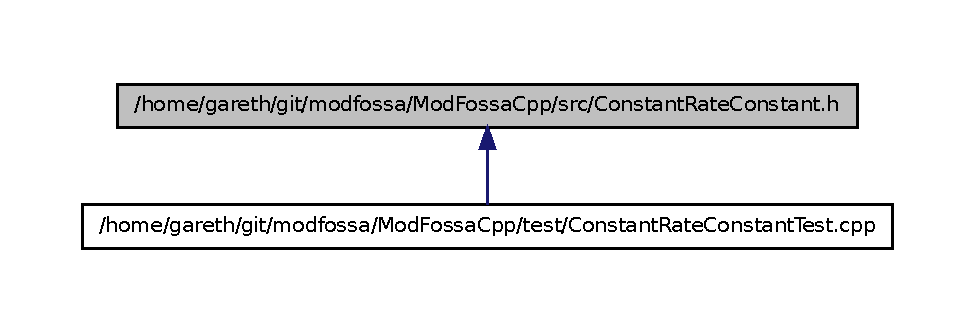
\includegraphics[width=400pt]{ConstantRateConstant_8h__dep__incl}
\end{center}
\end{figure}
\subsection*{Classes}
\begin{DoxyCompactItemize}
\item 
class \hyperlink{classConstantRateConstant}{ConstantRateConstant}
\end{DoxyCompactItemize}

\hypertarget{MarkovModel_8cpp}{
\section{/home/gareth/git/modfossa/ModFossaCpp/src/MarkovModel.cpp File Reference}
\label{MarkovModel_8cpp}\index{/home/gareth/git/modfossa/ModFossaCpp/src/MarkovModel.cpp@{/home/gareth/git/modfossa/ModFossaCpp/src/MarkovModel.cpp}}
}
{\ttfamily \#include \char`\"{}MarkovModel.h\char`\"{}}\par
Include dependency graph for MarkovModel.cpp:\nopagebreak
\begin{figure}[H]
\begin{center}
\leavevmode
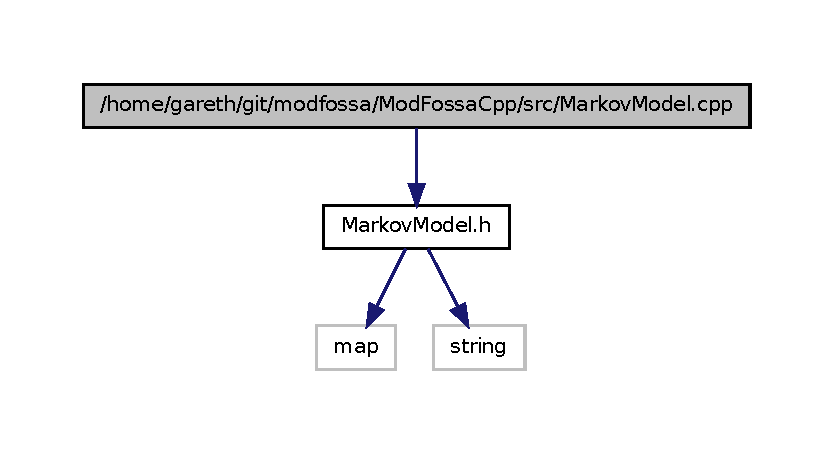
\includegraphics[width=400pt]{MarkovModel_8cpp__incl}
\end{center}
\end{figure}

\hypertarget{MarkovModel_8h}{
\section{/home/gareth/git/modfossa/ModFossaCpp/src/MarkovModel.h File Reference}
\label{MarkovModel_8h}\index{/home/gareth/git/modfossa/ModFossaCpp/src/MarkovModel.h@{/home/gareth/git/modfossa/ModFossaCpp/src/MarkovModel.h}}
}
{\ttfamily \#include $<$map$>$}\par
{\ttfamily \#include $<$string$>$}\par
Include dependency graph for MarkovModel.h:\nopagebreak
\begin{figure}[H]
\begin{center}
\leavevmode
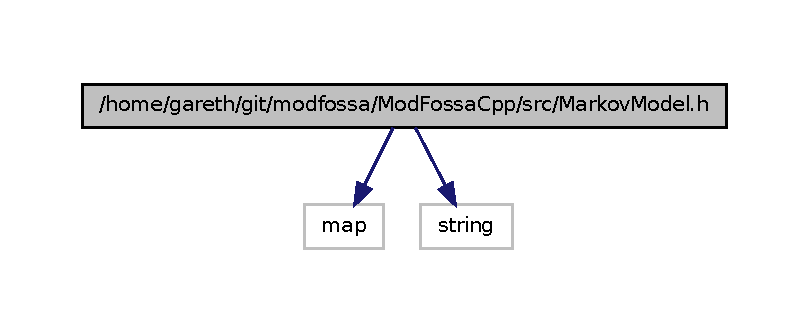
\includegraphics[width=388pt]{MarkovModel_8h__incl}
\end{center}
\end{figure}
This graph shows which files directly or indirectly include this file:\nopagebreak
\begin{figure}[H]
\begin{center}
\leavevmode
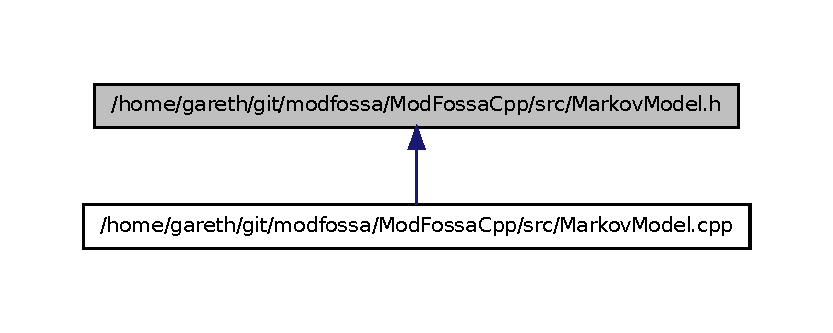
\includegraphics[width=400pt]{MarkovModel_8h__dep__incl}
\end{center}
\end{figure}
\subsection*{Classes}
\begin{DoxyCompactItemize}
\item 
class \hyperlink{classMarkovModel}{MarkovModel}
\begin{DoxyCompactList}\small\item\em Class responsible for creating and storing information required to describe a markov model for an ion channel. \item\end{DoxyCompactList}\end{DoxyCompactItemize}

\hypertarget{ModelDescription_8h}{
\section{/home/gareth/git/modfossa/ModFossaCpp/src/ModelDescription.h File Reference}
\label{ModelDescription_8h}\index{/home/gareth/git/modfossa/ModFossaCpp/src/ModelDescription.h@{/home/gareth/git/modfossa/ModFossaCpp/src/ModelDescription.h}}
}
{\ttfamily \#include $<$string$>$}\par
{\ttfamily \#include $<$vector$>$}\par
Include dependency graph for ModelDescription.h:\nopagebreak
\begin{figure}[H]
\begin{center}
\leavevmode
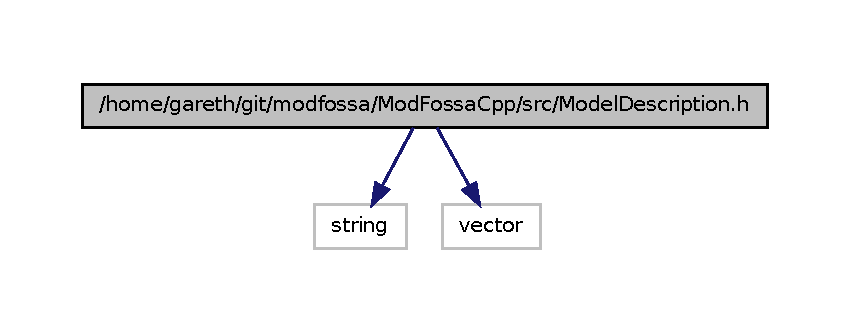
\includegraphics[width=400pt]{ModelDescription_8h__incl}
\end{center}
\end{figure}
\subsection*{Classes}
\begin{DoxyCompactItemize}
\item 
class \hyperlink{classModelDescription}{ModelDescription}
\end{DoxyCompactItemize}

\hypertarget{RateConstantBase_8cpp}{
\section{/home/gareth/git/modfossa/ModFossaCpp/src/RateConstantBase.cpp File Reference}
\label{RateConstantBase_8cpp}\index{/home/gareth/git/modfossa/ModFossaCpp/src/RateConstantBase.cpp@{/home/gareth/git/modfossa/ModFossaCpp/src/RateConstantBase.cpp}}
}
{\ttfamily \#include \char`\"{}RateConstantBase.h\char`\"{}}\par
Include dependency graph for RateConstantBase.cpp:\nopagebreak
\begin{figure}[H]
\begin{center}
\leavevmode
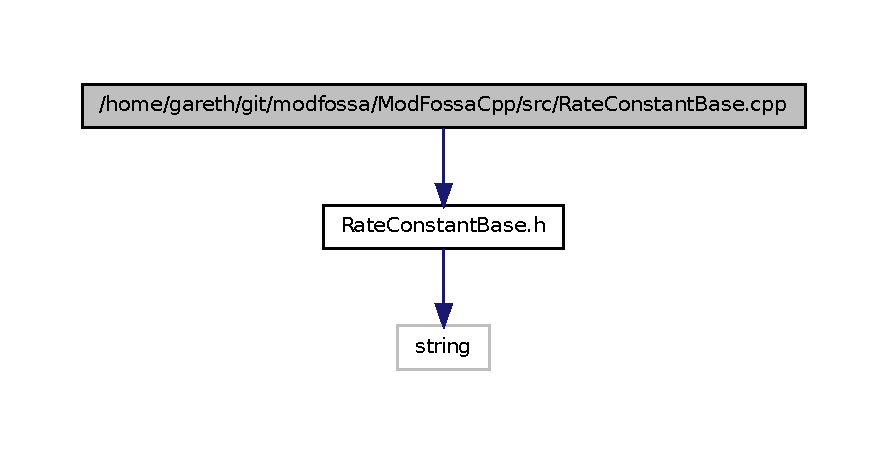
\includegraphics[width=400pt]{RateConstantBase_8cpp__incl}
\end{center}
\end{figure}

\hypertarget{RateConstantBase_8h}{
\section{/home/gareth/git/modfossa/ModFossaCpp/src/RateConstantBase.h File Reference}
\label{RateConstantBase_8h}\index{/home/gareth/git/modfossa/ModFossaCpp/src/RateConstantBase.h@{/home/gareth/git/modfossa/ModFossaCpp/src/RateConstantBase.h}}
}
{\ttfamily \#include $<$string$>$}\par
Include dependency graph for RateConstantBase.h:\nopagebreak
\begin{figure}[H]
\begin{center}
\leavevmode
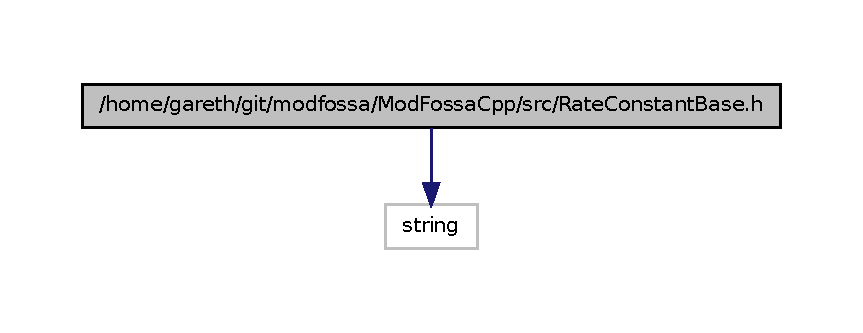
\includegraphics[width=400pt]{RateConstantBase_8h__incl}
\end{center}
\end{figure}
This graph shows which files directly or indirectly include this file:
\nopagebreak
\begin{figure}[H]
\begin{center}
\leavevmode
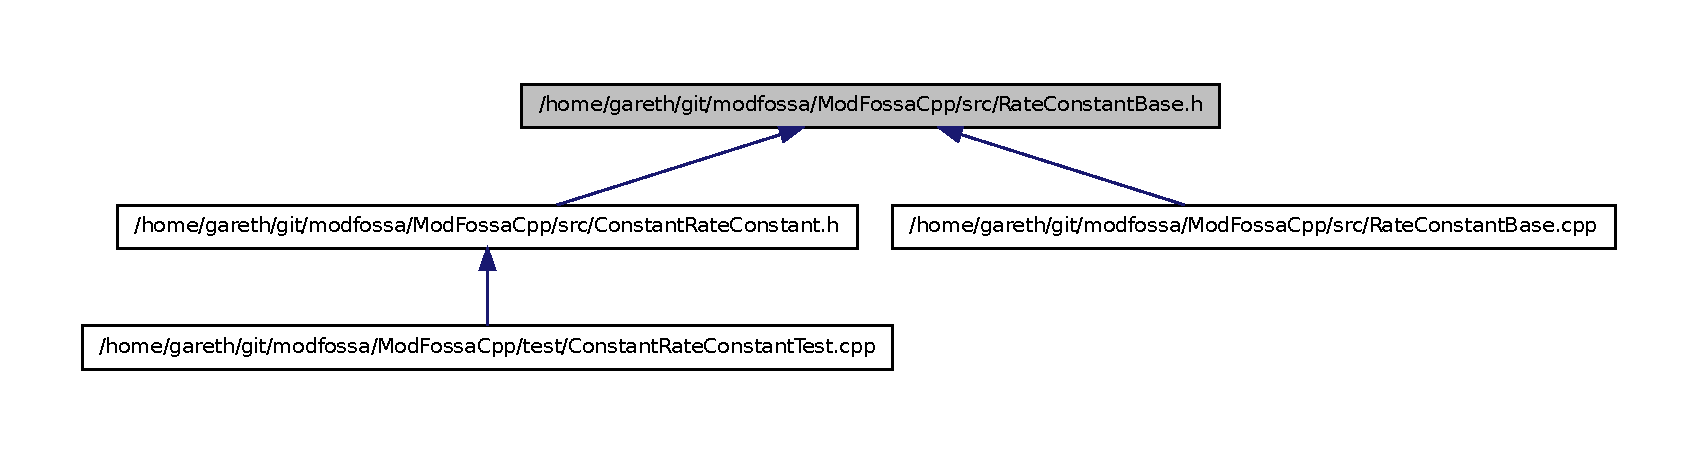
\includegraphics[width=400pt]{RateConstantBase_8h__dep__incl}
\end{center}
\end{figure}
\subsection*{Classes}
\begin{DoxyCompactItemize}
\item 
class \hyperlink{classRateConstantBase}{RateConstantBase}
\begin{DoxyCompactList}\small\item\em Abstract base class for RateConstants. \item\end{DoxyCompactList}\end{DoxyCompactItemize}

\hypertarget{RateConstantType_8h}{
\section{/home/gareth/git/modfossa/ModFossaCpp/src/RateConstantType.h File Reference}
\label{RateConstantType_8h}\index{/home/gareth/git/modfossa/ModFossaCpp/src/RateConstantType.h@{/home/gareth/git/modfossa/ModFossaCpp/src/RateConstantType.h}}
}
\subsection*{Enumerations}
\begin{DoxyCompactItemize}
\item 
enum \hyperlink{RateConstantType_8h_aa702a19181781068a67df2719eaea205}{RateConstantType} \{ \par
\hyperlink{RateConstantType_8h_aa702a19181781068a67df2719eaea205aaeefcc3671b16fd4226e51cfe73a8da7}{Constant}, 
\hyperlink{RateConstantType_8h_aa702a19181781068a67df2719eaea205a610e2d5c46142167481285863e9b8391}{Sigmoidal}, 
\hyperlink{RateConstantType_8h_aa702a19181781068a67df2719eaea205a6890237d462df8cb189355f4fc5d2f72}{LigandDependent}, 
\hyperlink{RateConstantType_8h_aa702a19181781068a67df2719eaea205af44a3f647fcbbd89fd3a0273e016ecd6}{Exponential}, 
\par
\hyperlink{RateConstantType_8h_aa702a19181781068a67df2719eaea205abb992010426acbe963b588344a83f33e}{Bolztmann}
 \}
\end{DoxyCompactItemize}


\subsection{Enumeration Type Documentation}
\hypertarget{RateConstantType_8h_aa702a19181781068a67df2719eaea205}{
\index{RateConstantType.h@{RateConstantType.h}!RateConstantType@{RateConstantType}}
\index{RateConstantType@{RateConstantType}!RateConstantType.h@{RateConstantType.h}}
\subsubsection[{RateConstantType}]{\setlength{\rightskip}{0pt plus 5cm}enum {\bf RateConstantType}}}
\label{RateConstantType_8h_aa702a19181781068a67df2719eaea205}
\begin{Desc}
\item[Enumerator: ]\par
\begin{description}
\index{Constant@{Constant}!RateConstantType.h@{RateConstantType.h}}\index{RateConstantType.h@{RateConstantType.h}!Constant@{Constant}}\item[{\em 
\hypertarget{RateConstantType_8h_aa702a19181781068a67df2719eaea205aaeefcc3671b16fd4226e51cfe73a8da7}{
Constant}
\label{RateConstantType_8h_aa702a19181781068a67df2719eaea205aaeefcc3671b16fd4226e51cfe73a8da7}
}]\index{Sigmoidal@{Sigmoidal}!RateConstantType.h@{RateConstantType.h}}\index{RateConstantType.h@{RateConstantType.h}!Sigmoidal@{Sigmoidal}}\item[{\em 
\hypertarget{RateConstantType_8h_aa702a19181781068a67df2719eaea205a610e2d5c46142167481285863e9b8391}{
Sigmoidal}
\label{RateConstantType_8h_aa702a19181781068a67df2719eaea205a610e2d5c46142167481285863e9b8391}
}]\index{LigandDependent@{LigandDependent}!RateConstantType.h@{RateConstantType.h}}\index{RateConstantType.h@{RateConstantType.h}!LigandDependent@{LigandDependent}}\item[{\em 
\hypertarget{RateConstantType_8h_aa702a19181781068a67df2719eaea205a6890237d462df8cb189355f4fc5d2f72}{
LigandDependent}
\label{RateConstantType_8h_aa702a19181781068a67df2719eaea205a6890237d462df8cb189355f4fc5d2f72}
}]\index{Exponential@{Exponential}!RateConstantType.h@{RateConstantType.h}}\index{RateConstantType.h@{RateConstantType.h}!Exponential@{Exponential}}\item[{\em 
\hypertarget{RateConstantType_8h_aa702a19181781068a67df2719eaea205af44a3f647fcbbd89fd3a0273e016ecd6}{
Exponential}
\label{RateConstantType_8h_aa702a19181781068a67df2719eaea205af44a3f647fcbbd89fd3a0273e016ecd6}
}]\index{Bolztmann@{Bolztmann}!RateConstantType.h@{RateConstantType.h}}\index{RateConstantType.h@{RateConstantType.h}!Bolztmann@{Bolztmann}}\item[{\em 
\hypertarget{RateConstantType_8h_aa702a19181781068a67df2719eaea205abb992010426acbe963b588344a83f33e}{
Bolztmann}
\label{RateConstantType_8h_aa702a19181781068a67df2719eaea205abb992010426acbe963b588344a83f33e}
}]\end{description}
\end{Desc}



Definition at line 4 of file RateConstantType.h.


\hypertarget{State_8cpp}{
\section{/home/gareth/git/modfossa/ModFossaCpp/src/State.cpp File Reference}
\label{State_8cpp}\index{/home/gareth/git/modfossa/ModFossaCpp/src/State.cpp@{/home/gareth/git/modfossa/ModFossaCpp/src/State.cpp}}
}
{\ttfamily \#include \char`\"{}State.h\char`\"{}}\par
Include dependency graph for State.cpp:\nopagebreak
\begin{figure}[H]
\begin{center}
\leavevmode
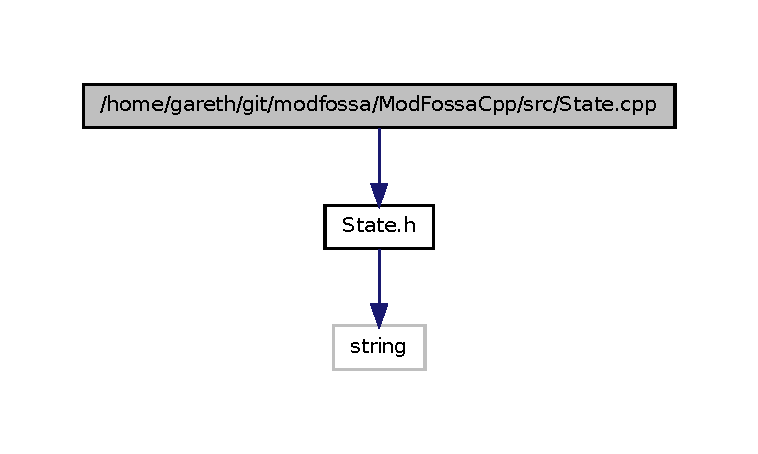
\includegraphics[width=364pt]{State_8cpp__incl}
\end{center}
\end{figure}

\hypertarget{State_8h}{
\section{/home/gareth/git/modfossa/ModFossaCpp/src/State.h File Reference}
\label{State_8h}\index{/home/gareth/git/modfossa/ModFossaCpp/src/State.h@{/home/gareth/git/modfossa/ModFossaCpp/src/State.h}}
}
{\ttfamily \#include $<$string$>$}\par
Include dependency graph for State.h:\nopagebreak
\begin{figure}[H]
\begin{center}
\leavevmode
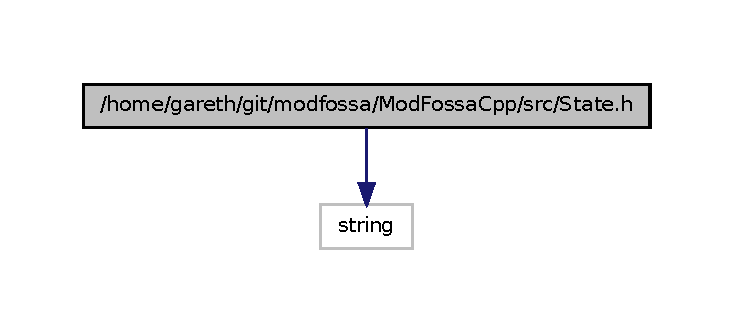
\includegraphics[width=352pt]{State_8h__incl}
\end{center}
\end{figure}
This graph shows which files directly or indirectly include this file:\nopagebreak
\begin{figure}[H]
\begin{center}
\leavevmode
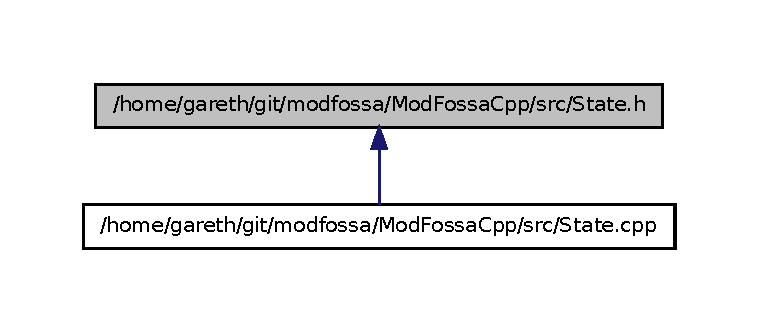
\includegraphics[width=364pt]{State_8h__dep__incl}
\end{center}
\end{figure}
\subsection*{Classes}
\begin{DoxyCompactItemize}
\item 
class \hyperlink{classState}{State}
\end{DoxyCompactItemize}

\hypertarget{StateOfTheWorld_8cpp}{
\section{/home/gareth/git/modfossa/ModFossaCpp/src/StateOfTheWorld.cpp File Reference}
\label{StateOfTheWorld_8cpp}\index{/home/gareth/git/modfossa/ModFossaCpp/src/StateOfTheWorld.cpp@{/home/gareth/git/modfossa/ModFossaCpp/src/StateOfTheWorld.cpp}}
}
{\ttfamily \#include \char`\"{}StateOfTheWorld.h\char`\"{}}\par
Include dependency graph for StateOfTheWorld.cpp:\nopagebreak
\begin{figure}[H]
\begin{center}
\leavevmode
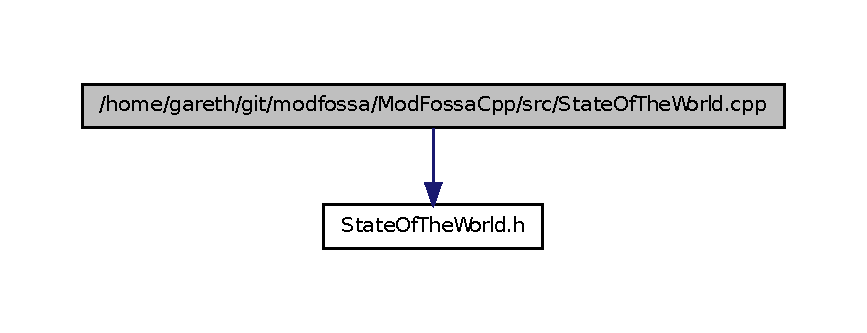
\includegraphics[width=400pt]{StateOfTheWorld_8cpp__incl}
\end{center}
\end{figure}

\hypertarget{StateOfTheWorld_8h}{
\section{/home/gareth/git/modfossa/ModFossaCpp/src/StateOfTheWorld.h File Reference}
\label{StateOfTheWorld_8h}\index{/home/gareth/git/modfossa/ModFossaCpp/src/StateOfTheWorld.h@{/home/gareth/git/modfossa/ModFossaCpp/src/StateOfTheWorld.h}}
}
This graph shows which files directly or indirectly include this file:\nopagebreak
\begin{figure}[H]
\begin{center}
\leavevmode
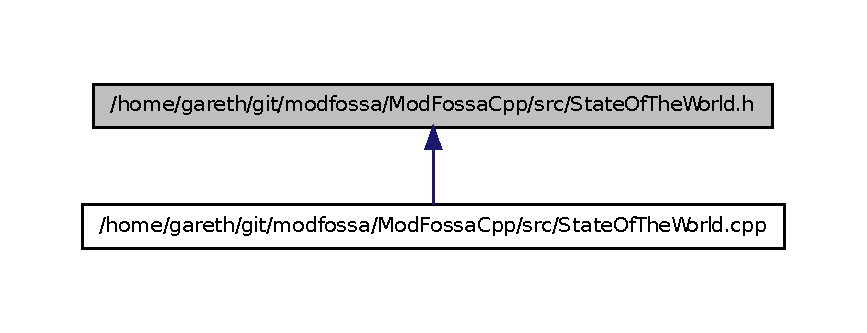
\includegraphics[width=400pt]{StateOfTheWorld_8h__dep__incl}
\end{center}
\end{figure}
\subsection*{Classes}
\begin{DoxyCompactItemize}
\item 
class \hyperlink{classStateOfTheWorld}{StateOfTheWorld}
\end{DoxyCompactItemize}

\hypertarget{ConstantRateConstantTest_8cpp}{
\section{/home/gareth/git/modfossa/ModFossaCpp/test/ConstantRateConstantTest.cpp File Reference}
\label{ConstantRateConstantTest_8cpp}\index{/home/gareth/git/modfossa/ModFossaCpp/test/ConstantRateConstantTest.cpp@{/home/gareth/git/modfossa/ModFossaCpp/test/ConstantRateConstantTest.cpp}}
}
{\ttfamily \#include \char`\"{}gtest/gtest.h\char`\"{}}\par
{\ttfamily \#include \char`\"{}../src/ConstantRateConstant.h\char`\"{}}\par
Include dependency graph for ConstantRateConstantTest.cpp:
\nopagebreak
\begin{figure}[H]
\begin{center}
\leavevmode
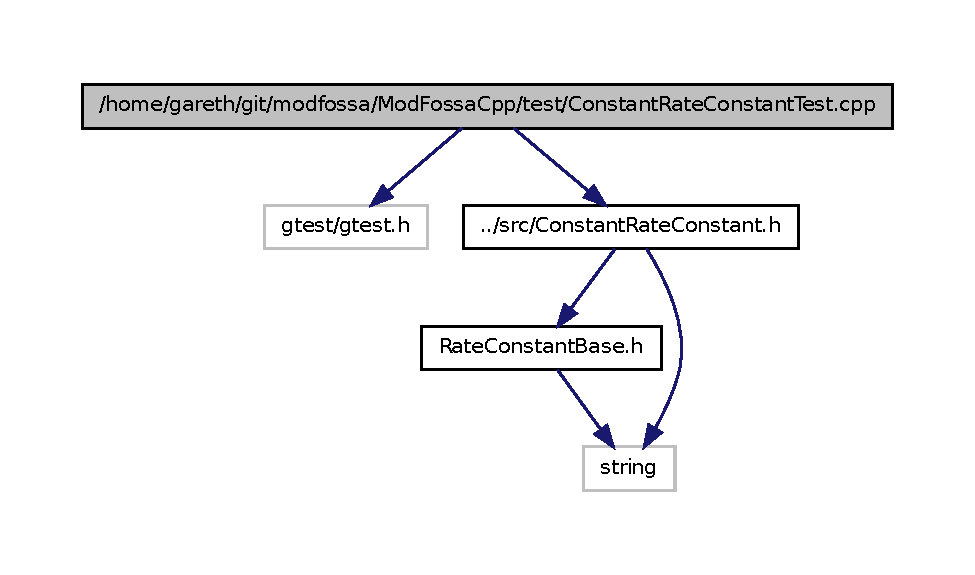
\includegraphics[width=400pt]{ConstantRateConstantTest_8cpp__incl}
\end{center}
\end{figure}
\subsection*{Classes}
\begin{DoxyCompactItemize}
\item 
class \hyperlink{classConstantRateConstantTest}{ConstantRateConstantTest}
\begin{DoxyCompactList}\small\item\em TestCase for ConstantRateContant. \item\end{DoxyCompactList}\end{DoxyCompactItemize}
\subsection*{Functions}
\begin{DoxyCompactItemize}
\item 
\hyperlink{ConstantRateConstantTest_8cpp_a5ee1bb9d6740c29fc1b214afafbed0cc}{TEST\_\-F} (\hyperlink{classConstantRateConstantTest}{ConstantRateConstantTest}, ConstructorValid)
\begin{DoxyCompactList}\small\item\em Test the parameterized constructor for valid input. \item\end{DoxyCompactList}\item 
\hyperlink{ConstantRateConstantTest_8cpp_aa7783e10d8a2c49936ed331404c179e6}{TEST\_\-F} (\hyperlink{classConstantRateConstantTest}{ConstantRateConstantTest}, ConstructorInvalidName)
\begin{DoxyCompactList}\small\item\em Test the parameterized constructor for invlaid name parameters. \item\end{DoxyCompactList}\end{DoxyCompactItemize}


\subsection{Function Documentation}
\hypertarget{ConstantRateConstantTest_8cpp_a5ee1bb9d6740c29fc1b214afafbed0cc}{
\index{ConstantRateConstantTest.cpp@{ConstantRateConstantTest.cpp}!TEST\_\-F@{TEST\_\-F}}
\index{TEST\_\-F@{TEST\_\-F}!ConstantRateConstantTest.cpp@{ConstantRateConstantTest.cpp}}
\subsubsection[{TEST\_\-F}]{\setlength{\rightskip}{0pt plus 5cm}TEST\_\-F (
\begin{DoxyParamCaption}
\item[{{\bf ConstantRateConstantTest}}]{, }
\item[{ConstructorValid}]{}
\end{DoxyParamCaption}
)}}
\label{ConstantRateConstantTest_8cpp_a5ee1bb9d6740c29fc1b214afafbed0cc}


Test the parameterized constructor for valid input. 



Definition at line 29 of file ConstantRateConstantTest.cpp.

\hypertarget{ConstantRateConstantTest_8cpp_aa7783e10d8a2c49936ed331404c179e6}{
\index{ConstantRateConstantTest.cpp@{ConstantRateConstantTest.cpp}!TEST\_\-F@{TEST\_\-F}}
\index{TEST\_\-F@{TEST\_\-F}!ConstantRateConstantTest.cpp@{ConstantRateConstantTest.cpp}}
\subsubsection[{TEST\_\-F}]{\setlength{\rightskip}{0pt plus 5cm}TEST\_\-F (
\begin{DoxyParamCaption}
\item[{{\bf ConstantRateConstantTest}}]{, }
\item[{ConstructorInvalidName}]{}
\end{DoxyParamCaption}
)}}
\label{ConstantRateConstantTest_8cpp_aa7783e10d8a2c49936ed331404c179e6}


Test the parameterized constructor for invlaid name parameters. 

Test the GetRate() method with valid StateOfTheWorld(). 

Definition at line 47 of file ConstantRateConstantTest.cpp.


\printindex
\end{document}
